\documentclass{article}
\usepackage[a4paper, paperwidth=25cm, paperheight=25.5cm, left=1.5cm, right=1.5cm, top=1cm, bottom=2cm]{geometry}
\usepackage{tikz,tcolorbox}
\usepackage{amsmath}
\usepackage[table,xcdraw]{xcolor}
\usepackage{listings}
\usepackage{array,multirow} % For customizing tables
\usepackage{booktabs} % For better horizontal lines
\usepackage{makecell}
\setlength{\parindent}{0pt}

\lstdefinestyle{sqlstyle}{
    language=SQL,                    % Set language to SQL
    basicstyle=\ttfamily\small,      % Font size and family for code
    keywordstyle=\color{blue}\bfseries, % Color for SQL keywords
    commentstyle=\color{gray},       % Color for comments
    stringstyle=\color{red},         % Color for strings
    numbers=left,                    % Show line numbers on the left
    numberstyle=\tiny\color{gray},   % Line number font and color
    stepnumber=1,                    % Line number step
    breaklines=true,                 % Wrap long lines
    frame=single,                    % Add a frame around code
    tabsize=2,                       % Set tab size
    showstringspaces=false           % Hide spaces in strings
}

\definecolor{commentgray}{HTML}{676160}
\definecolor{messagegreen}{HTML}{17B867}
\definecolor{myblue}{HTML}{10C2C4}

\tcbuselibrary{skins, breakable, theorems}


\newtcolorbox{prettyBox}[2]{
  enhanced,
  colback=white!90!#2,   % Background color based on the second parameter (color)
  colframe=#2!60!black,  % Frame color based on the second parameter (color)
  coltitle=white,        % Title color (white)
  fonttitle=\bfseries\Large,
  title=#1,              % Title from the first parameter
  boxrule=1mm,
  arc=0.5mm,
  drop shadow=#2!35!gray, % Drop shadow color based on the second parameter (color)
}

\setcellgapes{2pt}  % Adjust padding as needed
\makegapedcells


\begin{document}
\renewcommand{\arrayrulewidth}{0.75mm} % Set line thickness
\setlength{\tabcolsep}{10pt} % Set horizontal padding
\renewcommand{\arraystretch}{1} % Set vertical padding (1.0 is default)
\arrayrulecolor{myblue!70!black}

\subsection*{\underline{Partie 1}}
On doit d'abord se connecter en tant que system.

\lstinputlisting[style=sqlstyle]{SQL/Partie1/connect.sql}

\begin{center}
    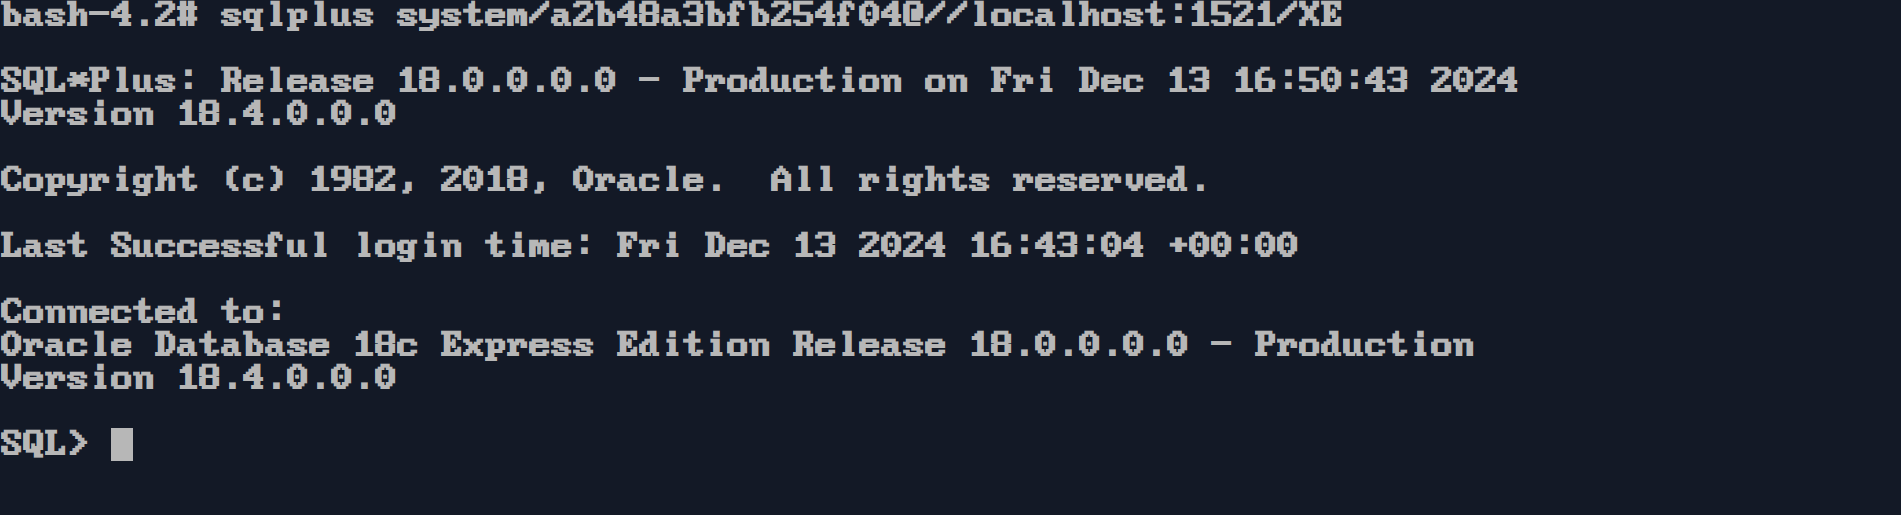
\includegraphics[width=\textwidth]{ScreenShot/Partie1/connect.png}
\end{center}



\vspace{0.25cm}
\subsubsection*{1.a}
Creation de la tablespace IOT\_TBS

\lstinputlisting[style=sqlstyle]{SQL/Partie1/ts1.sql}

\begin{center}
    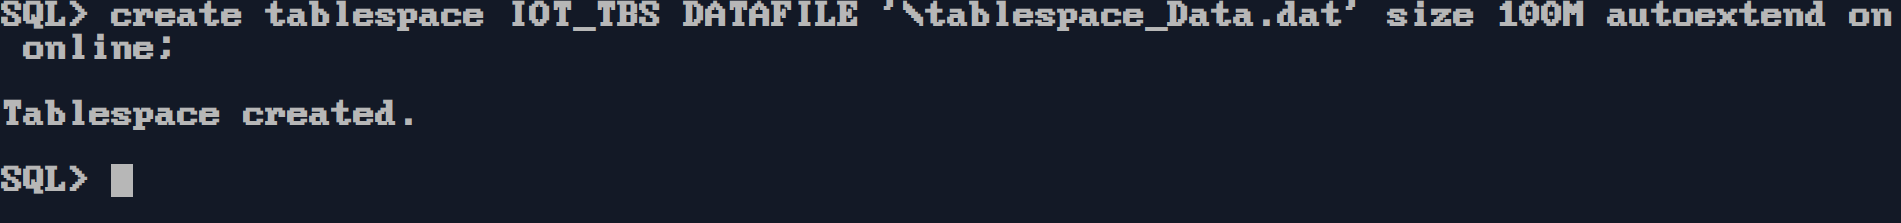
\includegraphics[width=\textwidth]{ScreenShot/Partie1/ts1.png}
\end{center}



\vspace{0.25cm}
\subsubsection*{1.b}
Creation de la tablespace temporaire IOT\_TempTBS

\lstinputlisting[style=sqlstyle]{SQL/Partie1/ts2.sql}

\begin{center}
    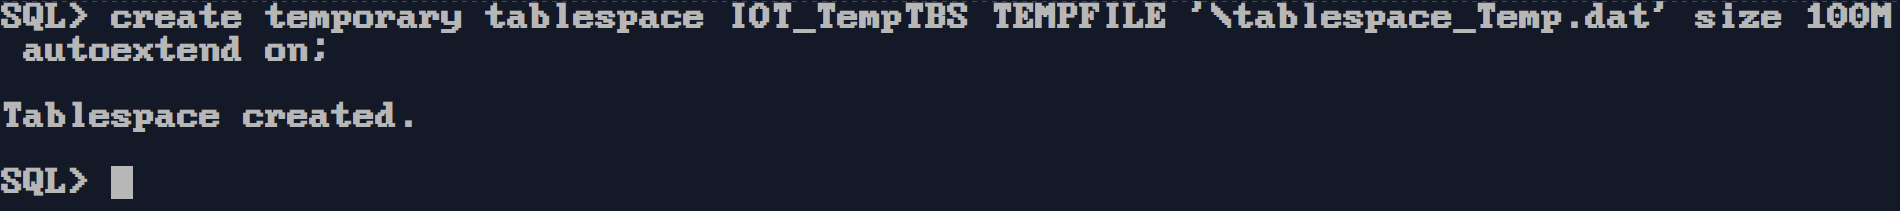
\includegraphics[width=\textwidth]{ScreenShot/Partie1/ts2.png}
\end{center}



\newpage
\subsubsection*{2.}

Création de l'utilisateur DBAIOT, en lui attribuant les tablespaces que nous avons créés et en définissant '1234' comme mot de passe.

\lstinputlisting[style=sqlstyle]{SQL/Partie1/dbaiot.sql}

\begin{center}
    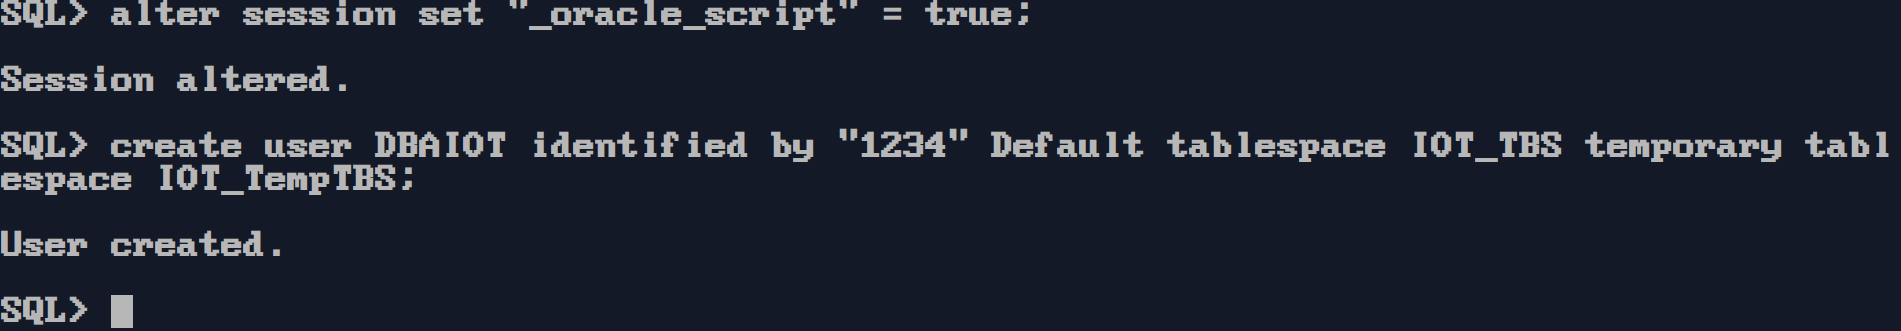
\includegraphics[width=\textwidth]{ScreenShot/Partie1/dbaiot.png}
\end{center}



\vspace{0.25cm}
\subsubsection*{3.}
On donne tous les droits et privilèges à l'utilisateur DBAIOT.

\lstinputlisting[style=sqlstyle]{SQL/Partie1/grant.sql}

\begin{center}
    
\includegraphics[width=\textwidth]{ScreenShot/Partie1/grant.png}
\end{center}



\vspace{0.25cm}
\subsection*{\underline{Partie 2}}
On doit d'abord se connecter en tant que system.

\lstinputlisting[style=sqlstyle]{SQL/Partie1/connect.sql}

\begin{center}
    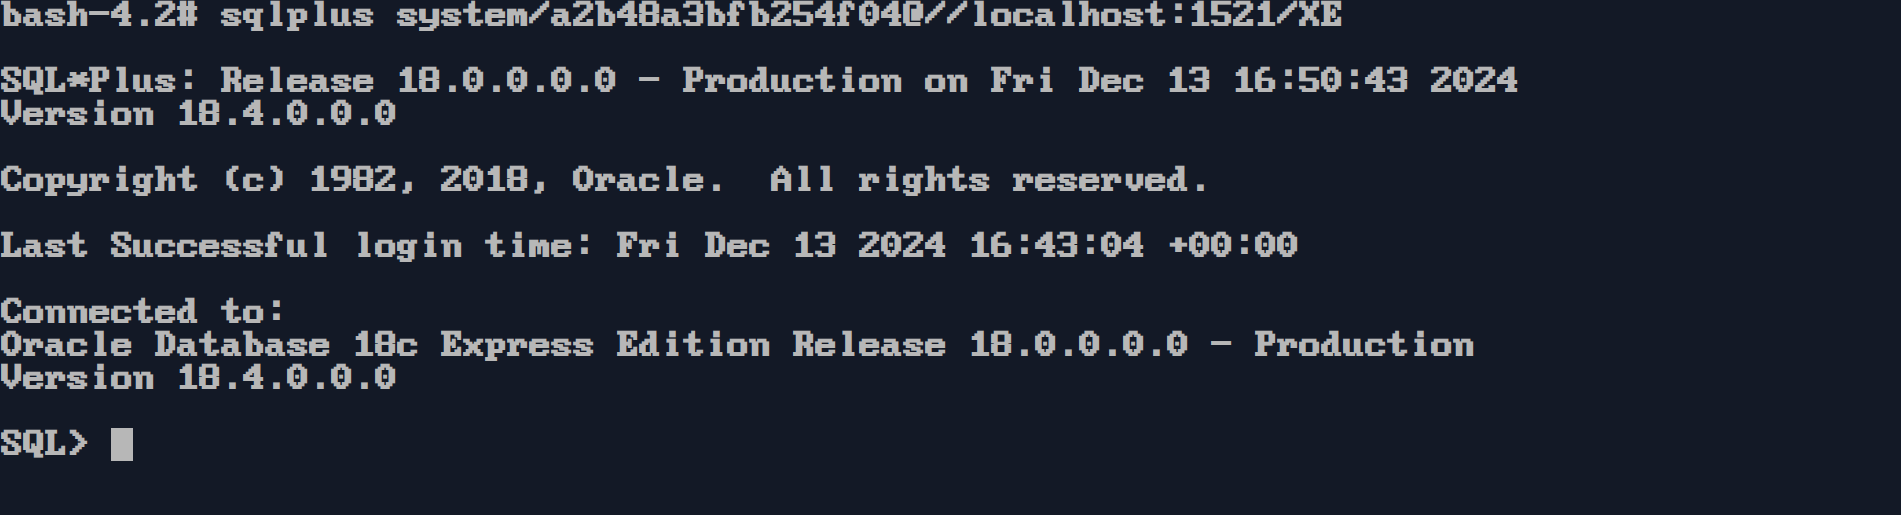
\includegraphics[width=\textwidth]{ScreenShot/Partie1/connect.png}
\end{center}



\vspace{0.25cm}
\subsubsection*{1.a}
Creation de la table users 

\lstinputlisting[style=sqlstyle]{SQL/Partie2/createTable/users.sql}

\begin{center}
    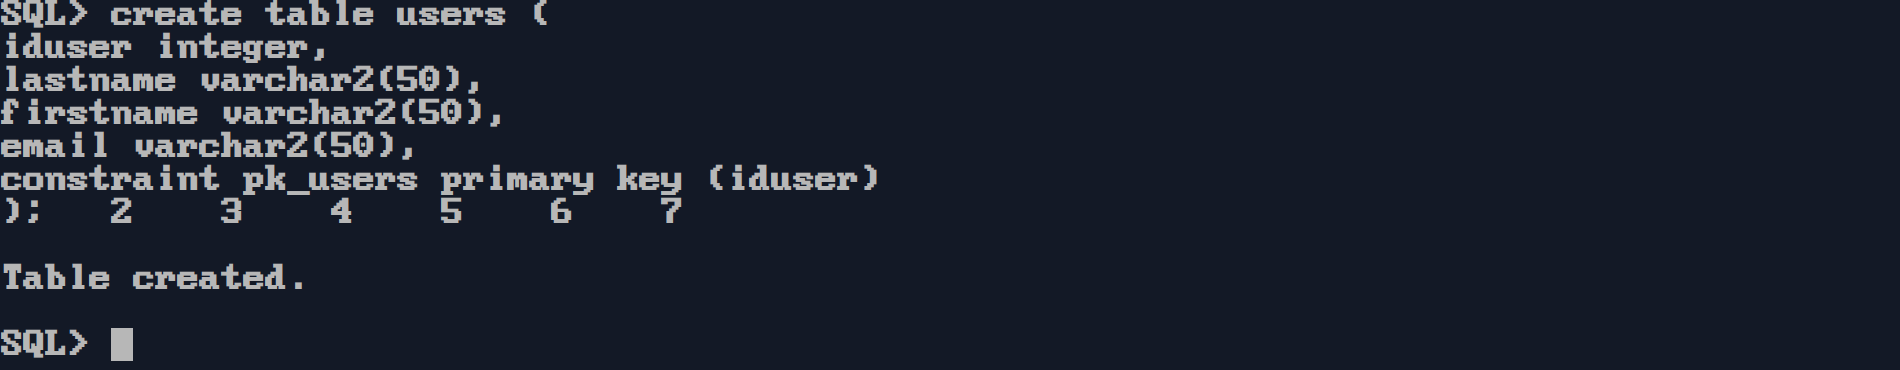
\includegraphics[width=\textwidth]{ScreenShot/Partie2/createTable/users.png}
\end{center}

\vspace{0.25cm}
\subsubsection*{1.b}
Creation de la table service 

\lstinputlisting[style=sqlstyle]{SQL/Partie2/createTable/service.sql}

\begin{center}
    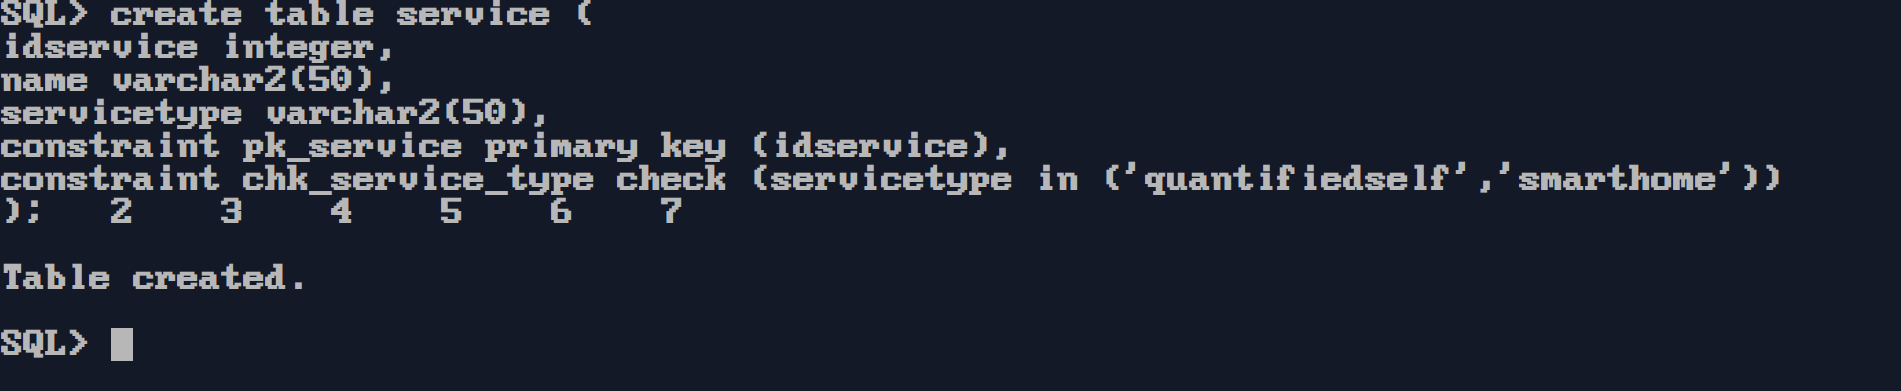
\includegraphics[width=\textwidth]{ScreenShot/Partie2/createTable/service.png}
\end{center}

\newpage
\subsubsection*{1.c}
Creation de la table thing 

\lstinputlisting[style=sqlstyle]{SQL/Partie2/createTable/thing.sql}

\begin{center}
    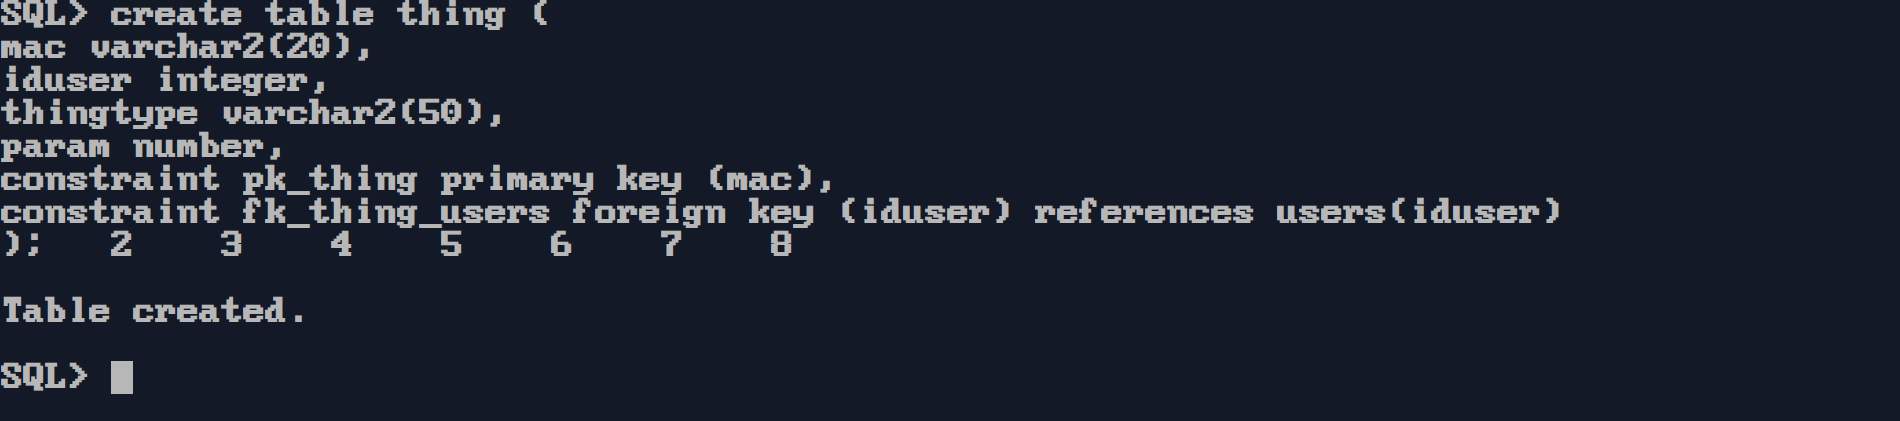
\includegraphics[width=\textwidth]{ScreenShot/Partie2/createTable/thing.png}
\end{center}


\vspace{0.25cm}
\subsubsection*{1.d}
Creation de la table subscribe

\lstinputlisting[style=sqlstyle]{SQL/Partie2/createTable/sub.sql}

\begin{center}
    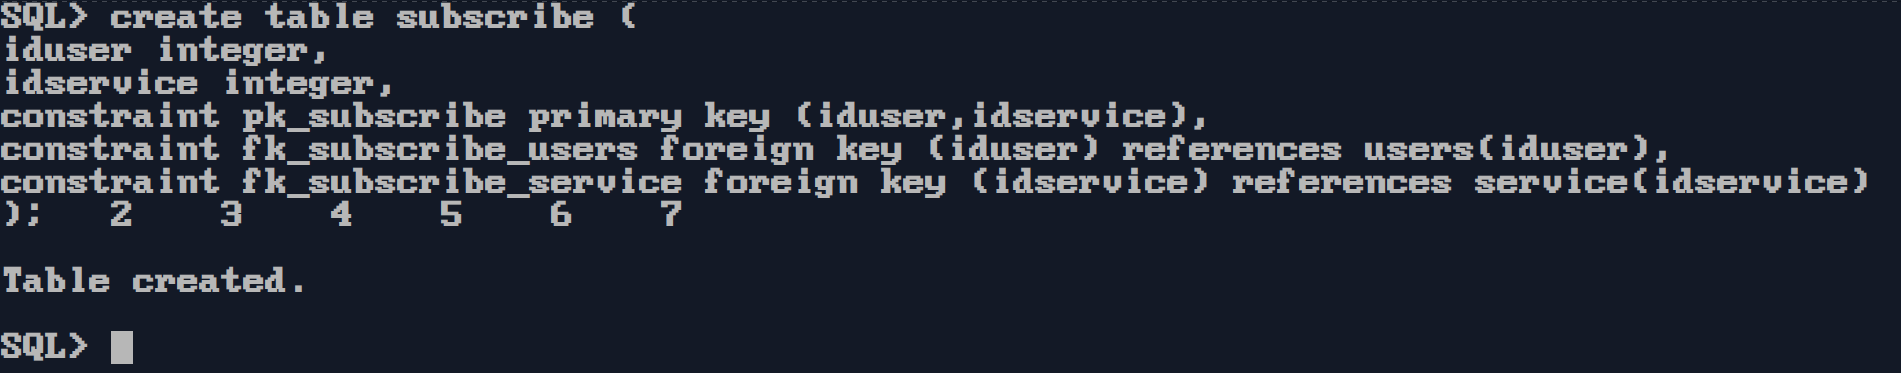
\includegraphics[width=\textwidth]{ScreenShot/Partie2/createTable/sub.png}
\end{center}





\newpage
\subsubsection*{2.}
Ajouter l'attribut adressuser de la table users 

\lstinputlisting[style=sqlstyle]{SQL/Partie2/addCol.sql}

\begin{center}
    
\includegraphics[width=\textwidth]{ScreenShot/Partie2/addCol.png}
\end{center}




\vspace{0.25cm}
\subsubsection*{3.a}
Ajouter la contrainte not null pour l'attribut lastname de la table users

\lstinputlisting[style=sqlstyle]{SQL/Partie2/nn1.sql}

\begin{center}
    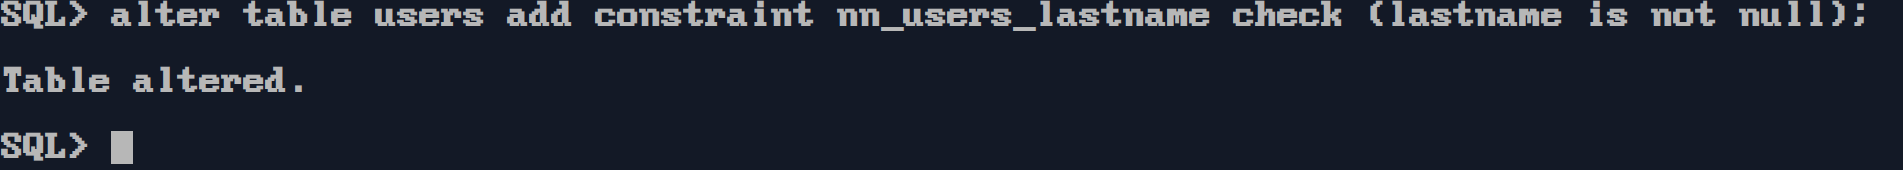
\includegraphics[width=\textwidth]{ScreenShot/Partie2/nn1.png}
\end{center}

\vspace{0.25cm}
\subsubsection*{3.b}
Ajouter la contrainte not null pour l'attribut adressuser de la table users

\lstinputlisting[style=sqlstyle]{SQL/Partie2/nn2.sql}

\begin{center}
    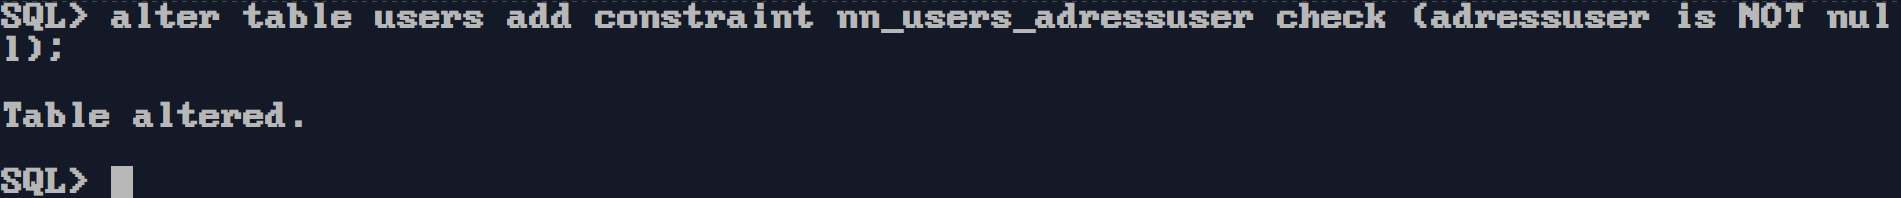
\includegraphics[width=\textwidth]{ScreenShot/Partie2/nn2.png}
\end{center}


\vspace{0.25cm}
\subsubsection*{4.a}
Agrandir la taille de l'attribut adressuser de la table users

\lstinputlisting[style=sqlstyle]{SQL/Partie2/big.sql}

\begin{center}
    
\includegraphics[width=\textwidth]{ScreenShot/Partie2/big.png}
\end{center}

\vspace{0.25cm}
\subsubsection*{4.b}
Reduire la taille de l'attribut adressuser de la table users

\lstinputlisting[style=sqlstyle]{SQL/Partie2/small.sql}

\begin{center}
    
\includegraphics[width=\textwidth]{ScreenShot/Partie2/small.png}
\end{center}


\vspace{0.25cm}
\subsubsection*{5.a}
Renommer l'attribut adressuser de la table users a adruser

\lstinputlisting[style=sqlstyle]{SQL/Partie2/rename.sql}

\begin{center}
    
\includegraphics[width=\textwidth]{ScreenShot/Partie2/rename.png}
\end{center}

\vspace{0.25cm}
\subsubsection*{5.b}
On verifie le changement du nom en utilisant desc pour afficher la structure de la table

\lstinputlisting[style=sqlstyle]{SQL/Partie2/verifyrename.sql}

\begin{center}
    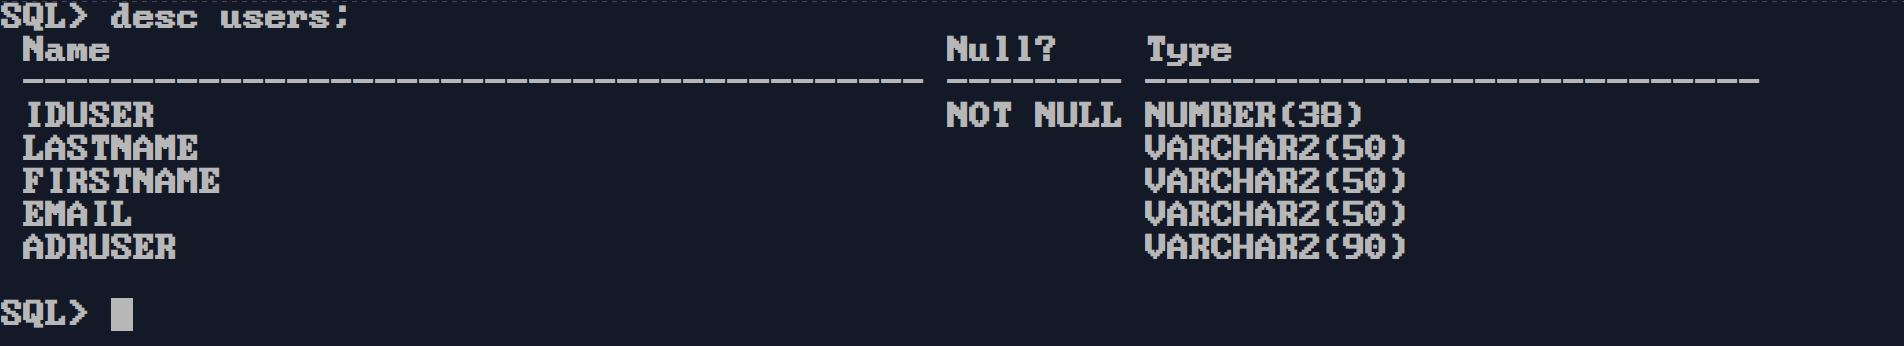
\includegraphics[width=\textwidth]{ScreenShot/Partie2/verifyrename.png}
\end{center}



\vspace{0.25cm}
\subsubsection*{6.a}
Supprimer l'attribut adruser de la table users

\lstinputlisting[style=sqlstyle]{SQL/Partie2/drop.sql}

\begin{center}
    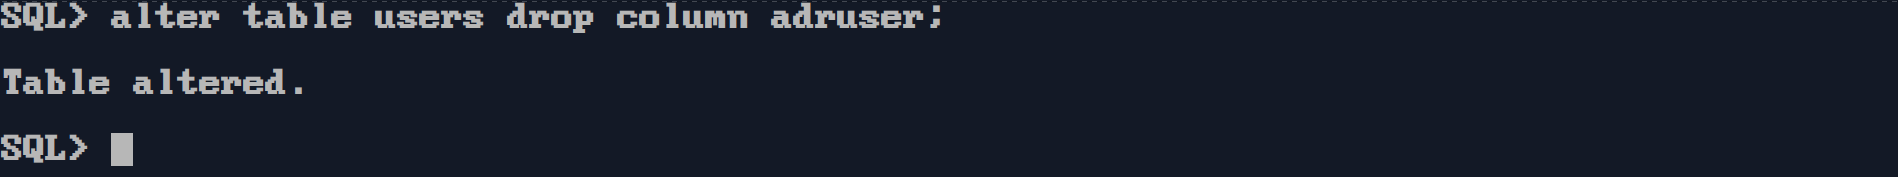
\includegraphics[width=\textwidth]{ScreenShot/Partie2/drop.png}
\end{center}

\vspace{0.25cm}
\subsubsection*{6.b}
On verifie la suppression de l'attribut adruser utilisant desc pour afficher la structure de la table

\lstinputlisting[style=sqlstyle]{SQL/Partie2/verifydrop.sql}

\begin{center}
    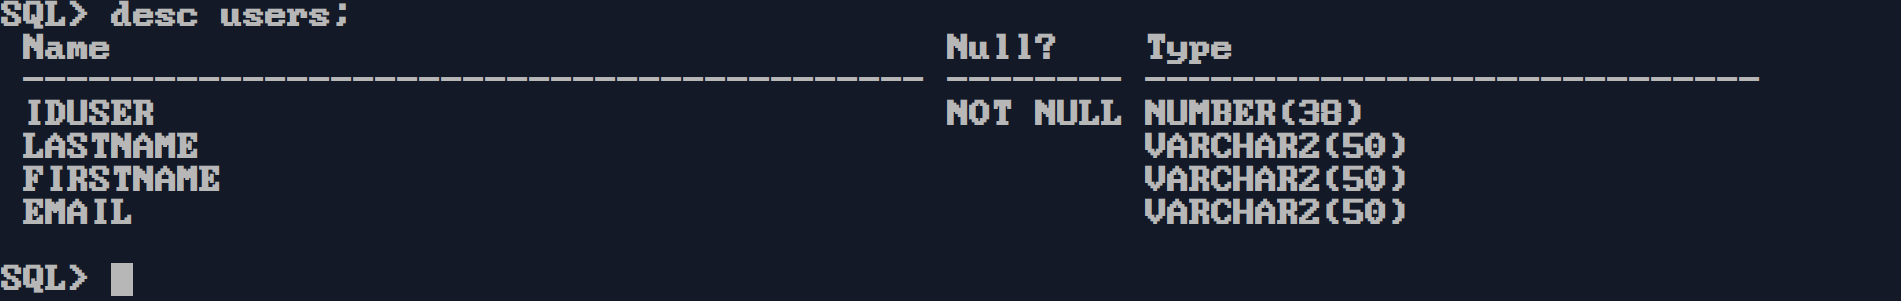
\includegraphics[width=\textwidth]{ScreenShot/Partie2/verifydrop.png}
\end{center}


\vspace{0.25cm}
\subsubsection*{7.}
Pour reprondre a ce besoin on doit ajouter les deux attributs date\_fin et date\_deb a la table subscribe

\vspace{0.25cm}
\subsubsection*{7.a}
Ajouter l'attribut date\_deb, supprimer l'ancienne contrainte pk\_subscribe, puis la recréer en incluant date\_deb dans la clé primaire de la table subscribe.
\lstinputlisting[style=sqlstyle]{SQL/Partie2/deb.sql}

\begin{center}
    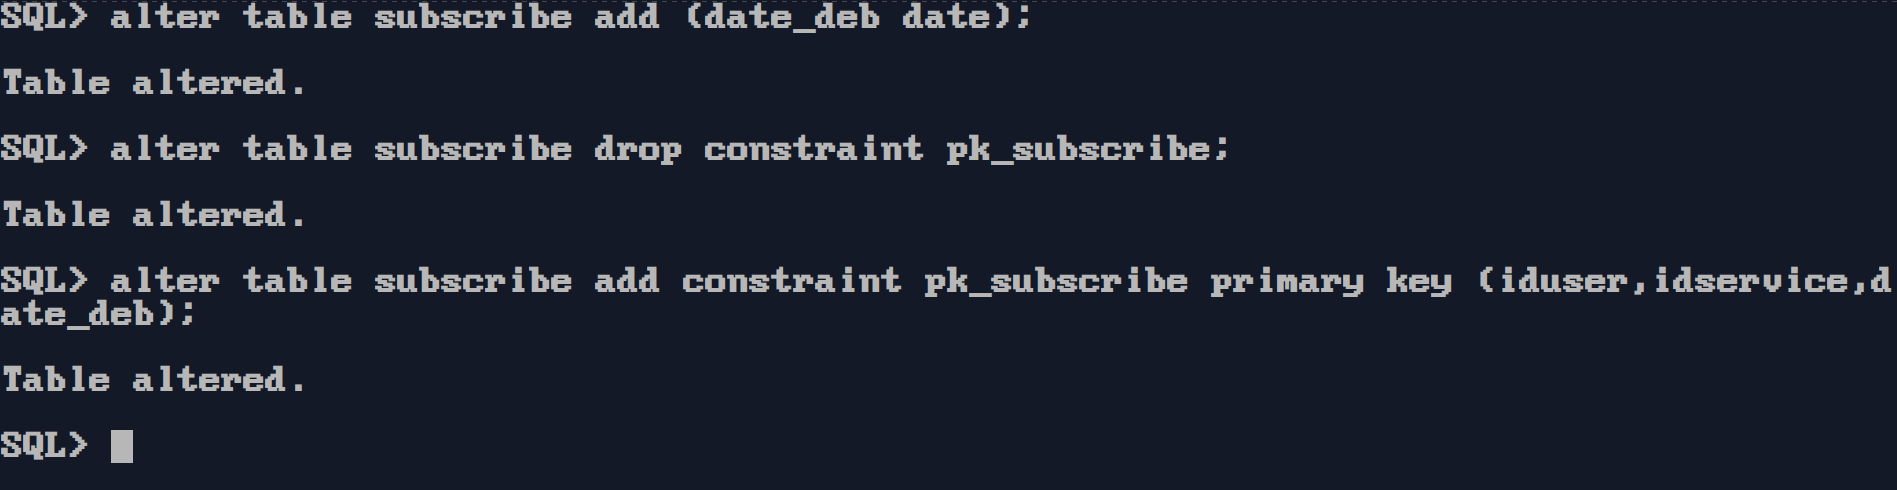
\includegraphics[width=\textwidth]{ScreenShot/Partie2/deb.png}
\end{center}

\newpage
\subsubsection*{7.b}
Ajouter l'attribut date\_fin et ajouter une contrainte pour verifie que date\_deb\(<\)date\_fin

\lstinputlisting[style=sqlstyle]{SQL/Partie2/fin.sql}

\begin{center}
    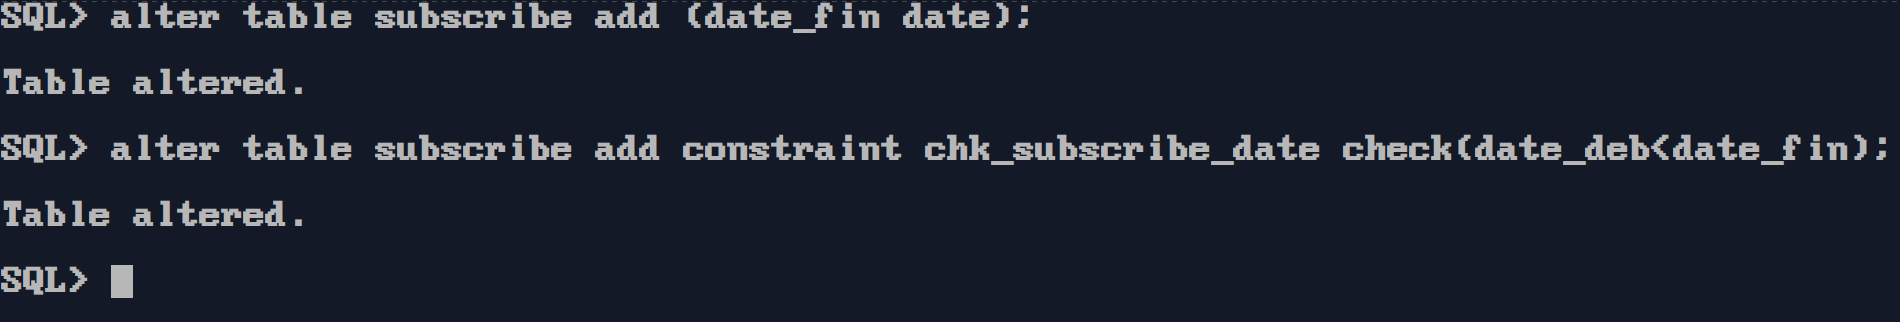
\includegraphics[width=\textwidth]{ScreenShot/Partie2/fin.png}
\end{center}


\vspace{0.25cm}
\subsection*{\underline{Partie 3}}
\subsection*{Insert}
All insert queries are inside SQL/EX2/insert folder



\vspace{0.25cm}
\subsection*{\underline{Partie 4}}
\subsubsection*{1.}

Création de l'utilisateur Admin, en lui attribuant les tablespaces que nous avons créés et en définissant '1234' comme mot de passe.

\lstinputlisting[style=sqlstyle]{SQL/Partie4/admin.sql}

\begin{center}
    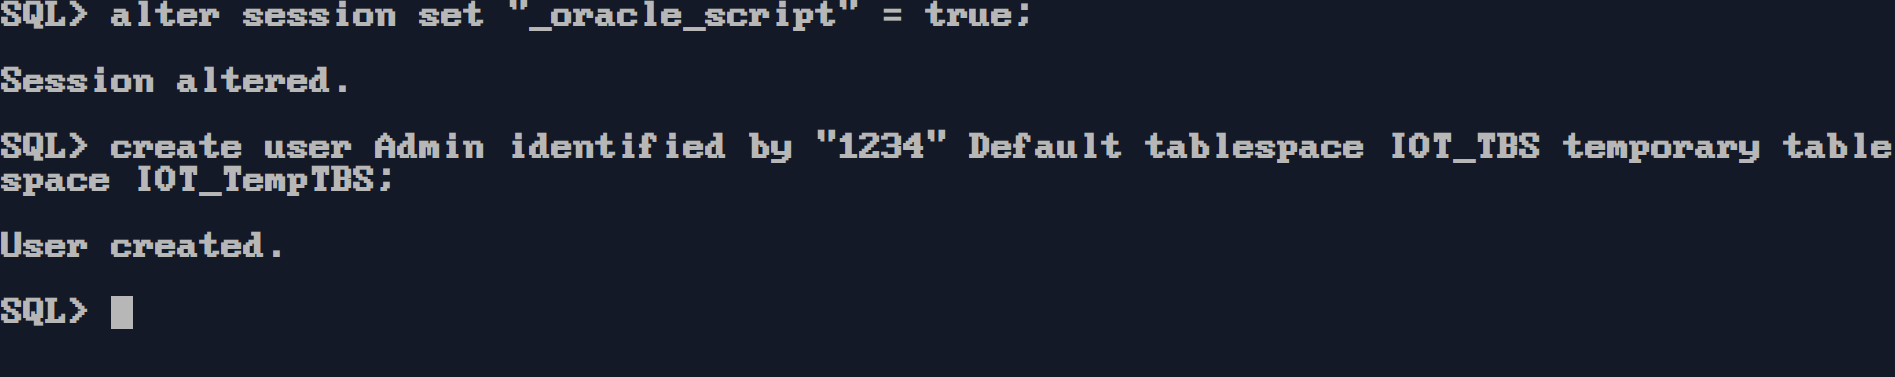
\includegraphics[width=\textwidth]{ScreenShot/Partie4/admin.png}
\end{center}




\newpage
On doit d'abord se connecter en tant que system.

\lstinputlisting[style=sqlstyle]{SQL/Partie1/connect.sql}

\begin{center}
    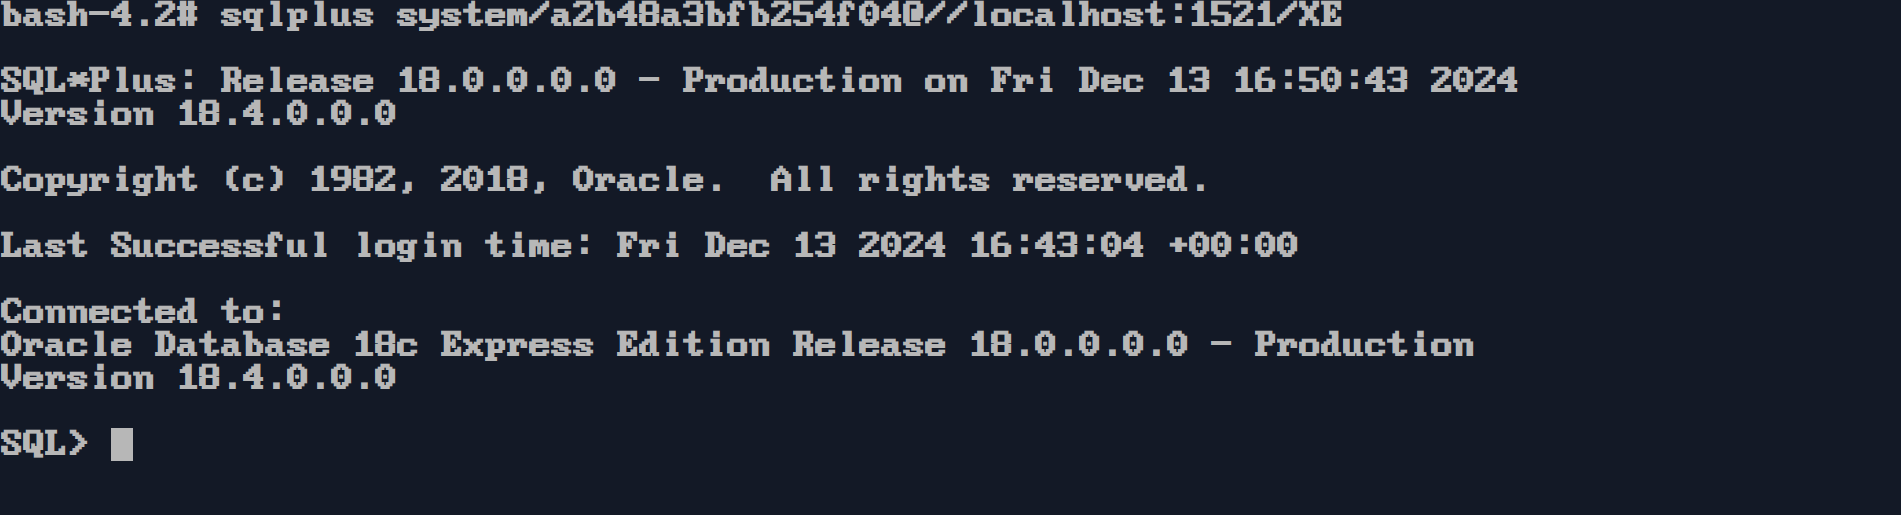
\includegraphics[width=\textwidth]{ScreenShot/Partie1/connect.png}
\end{center}



\vspace{0.25cm}
\subsubsection*{3.a}
On donne le droit de créer une session a admin depuis DBAIOT

\lstinputlisting[style=sqlstyle]{SQL/Partie4/grantsession.sql}

\begin{center}
    
\includegraphics[width=\textwidth]{ScreenShot/Partie4/grantsession.png}
\end{center}

\subsubsection*{3.b}
On se connecte en tant que admin.

\lstinputlisting[style=sqlstyle]{SQL/Partie4/connect.sql}

\begin{center}
    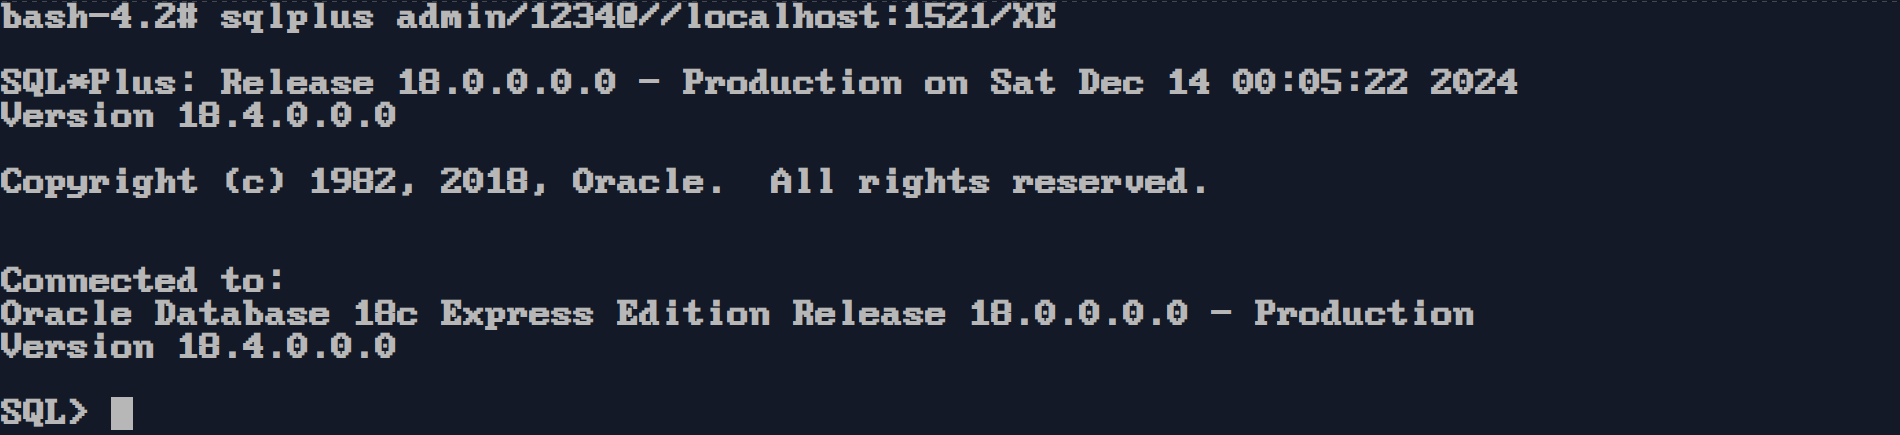
\includegraphics[width=\textwidth]{ScreenShot/Partie4/connect2.png}
\end{center}




\vspace{0.25cm}
\subsubsection*{4.a}
On donne le droit de créer des tables et utilisateurs a admin depuis DBAIOT

\lstinputlisting[style=sqlstyle]{SQL/Partie4/grant1.sql}

\begin{center}
    
\includegraphics[width=\textwidth]{ScreenShot/Partie4/grant1.png}
\end{center}

\subsubsection*{4.b}
Pour verifie les droit de admin on va afficher la table USER\_SYS\_PRIVS 

\lstinputlisting[style=sqlstyle]{SQL/Partie4/verify1.sql}

\begin{center}
    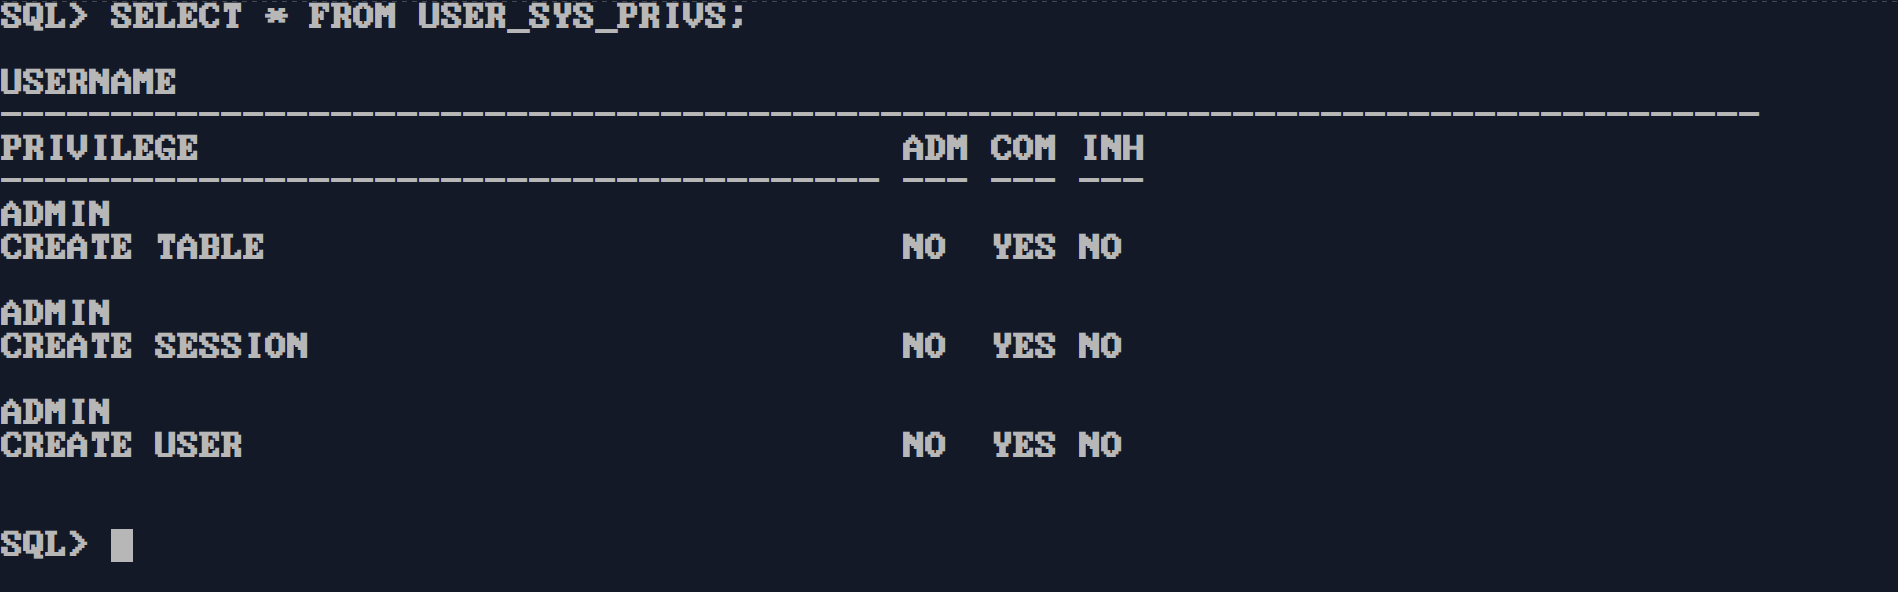
\includegraphics[width=\textwidth]{ScreenShot/Partie4/verify1.png}
\end{center}

\begin{prettyBox}{Remarque}{myblue}
La table USER\_SYS\_PRIVS affiche les privilèges du user avec lequel on
est connecté. La colonne ADM (admin) indique que l'utilisateur peut accorder 
ou révoquer ce privilège, COM (command) signifie que l'utilisateur a droit
à ce privilège, et INH (inherit) indique que l'utilisateur a obtenu ce privilège 
indirectement via un role.
\end{prettyBox}



\newpage
\subsubsection*{5.}
On va executer \textbf{Q1} depuis admin

\lstinputlisting[style=sqlstyle]{SQL/Partie4/select.sql}

\begin{center}
    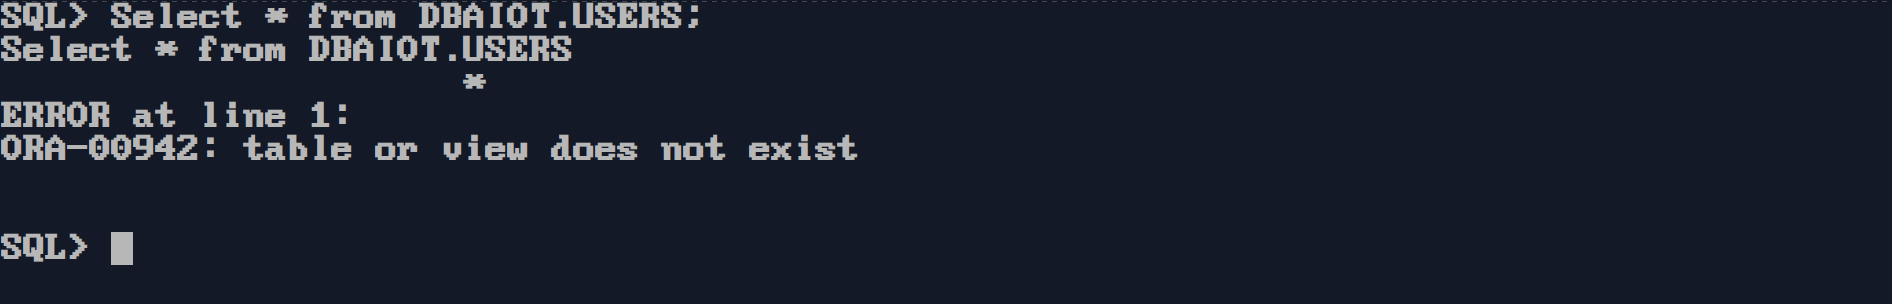
\includegraphics[width=\textwidth]{ScreenShot/Partie4/select.png}
\end{center}

\begin{prettyBox}{}{myblue}
Le problem est que l'utilisateur admin n'a pas le privilege de selectionner la table DBAIOT.USERS 
\end{prettyBox}




\vspace{0.25cm}
\subsubsection*{6.a}
On donne le privelege de selectionner la table DBAIOT.USERS a admin depuis DBAIOT
On va executer \textbf{Q1} depuis admin

\lstinputlisting[style=sqlstyle]{SQL/Partie4/grantselect.sql}

\begin{center}
    
\includegraphics[width=\textwidth]{ScreenShot/Partie4/grantselect.png}
\end{center}

\subsubsection*{6.b}
On va executer \textbf{Q1} depuis admin

\lstinputlisting[style=sqlstyle]{SQL/Partie4/select.sql}

\begin{center}
    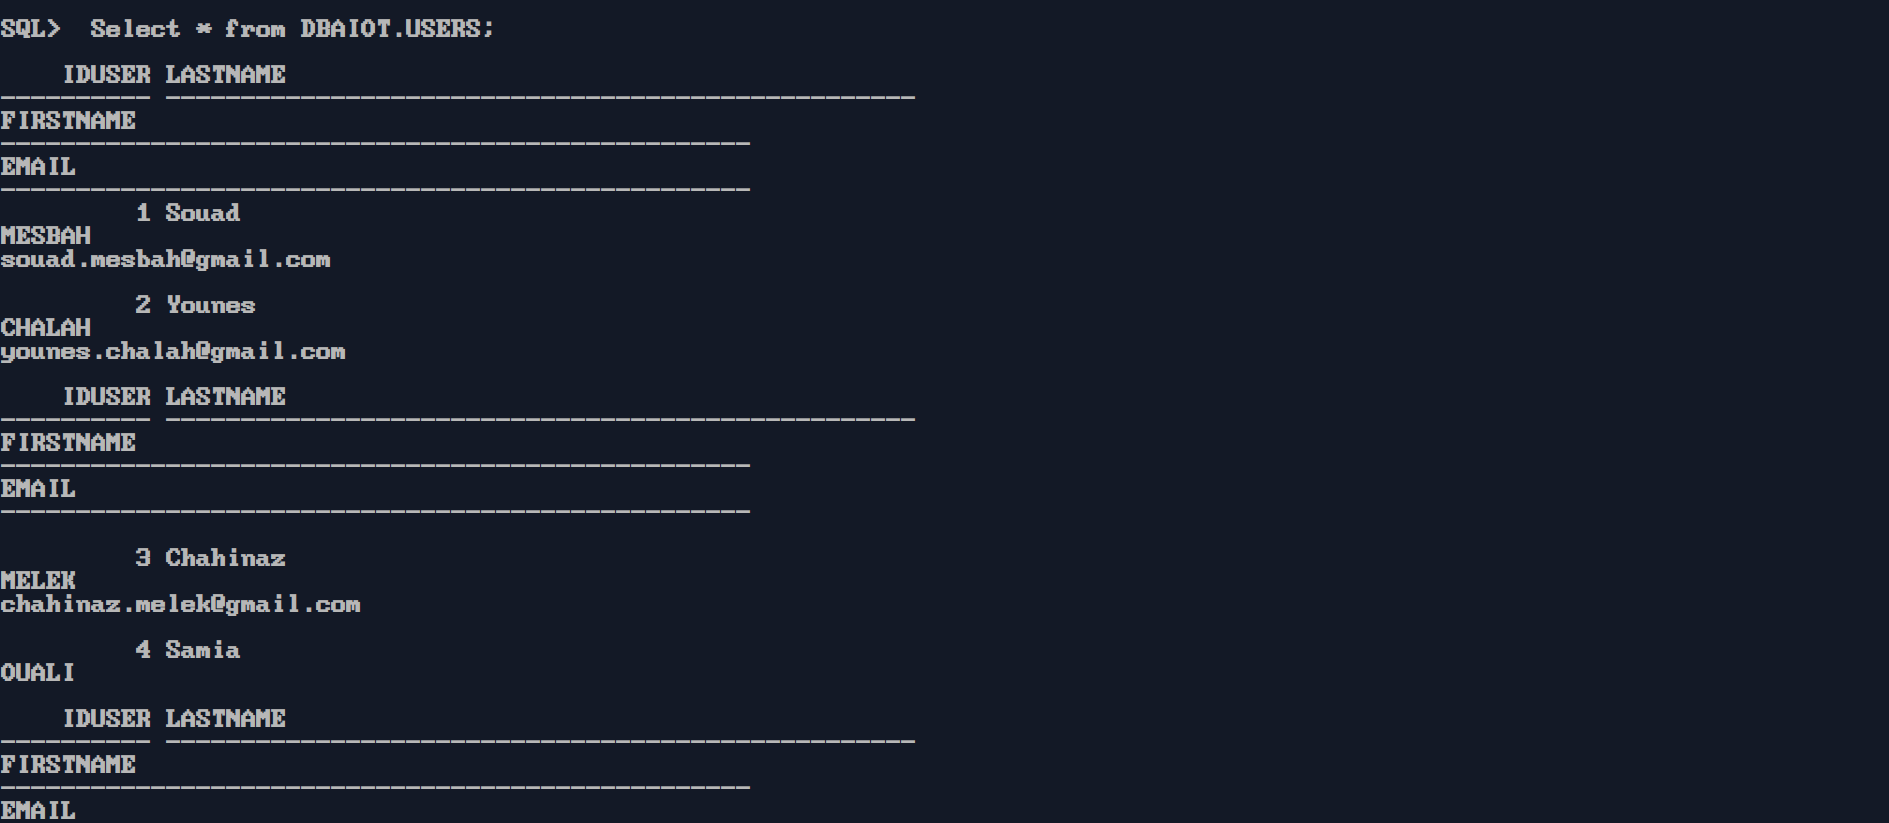
\includegraphics[width=\textwidth]{ScreenShot/Partie4/select1.png}
\end{center}




\vspace{0.25cm}
\subsubsection*{7.}
On va créer la vue USER\_THING avec une jointure entre les tables DBAIOT.USERS et DBAIOT.THING depuis l'utilisateur admin

\lstinputlisting[style=sqlstyle]{SQL/Partie4/createView.sql}

\begin{center}
    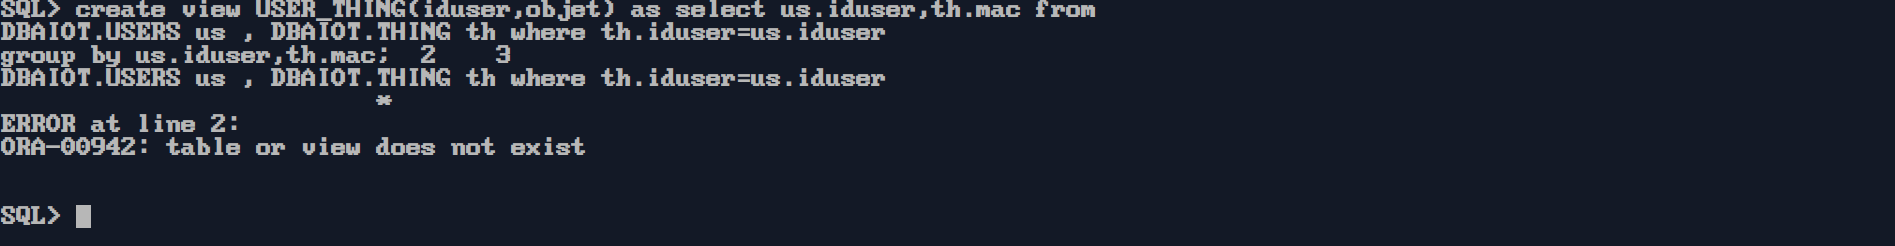
\includegraphics[width=\textwidth]{ScreenShot/Partie4/createView.png}
\end{center}

\begin{prettyBox}{}{myblue}
Le problem est que l'admin n'a pas le privelege de select la table DBAIOT.THING ni le privelge de creer des views
\end{prettyBox}


\vspace{0.25cm}
\subsubsection*{8.a}
On donne le droit de créer des view et selectionner la table DBAIOT.THING a admin depuis DBAIOT

\lstinputlisting[style=sqlstyle]{SQL/Partie4/grant2.sql}

\begin{center}
    
\includegraphics[width=\textwidth]{ScreenShot/Partie4/grant2.png}
\end{center}

\subsubsection*{8.b}
Creation de la vue USER\_THING depuis admin

\lstinputlisting[style=sqlstyle]{SQL/Partie4/createView.sql}

\begin{center}
    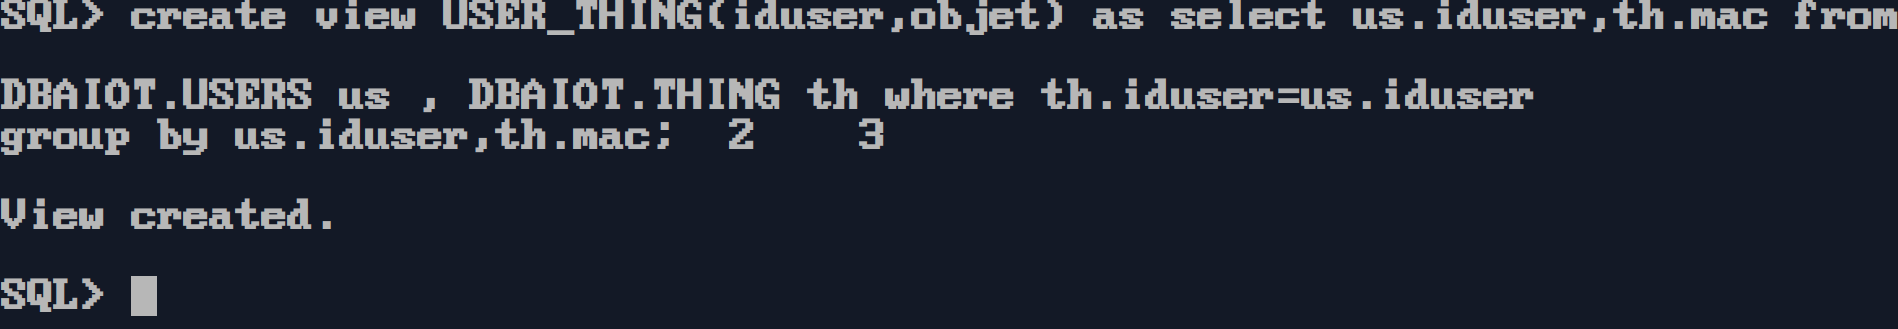
\includegraphics[width=\textwidth]{ScreenShot/Partie4/createView1.png}
\end{center}




\vspace{0.25cm}
\subsubsection*{9.}
On va créer l'index NAMESERVICE\_IX sur l’attribut NAME de la table DBAIOT.SERVICE depuis l'utilisateur admin

\lstinputlisting[style=sqlstyle]{SQL/Partie4/index.sql}

\begin{center}
    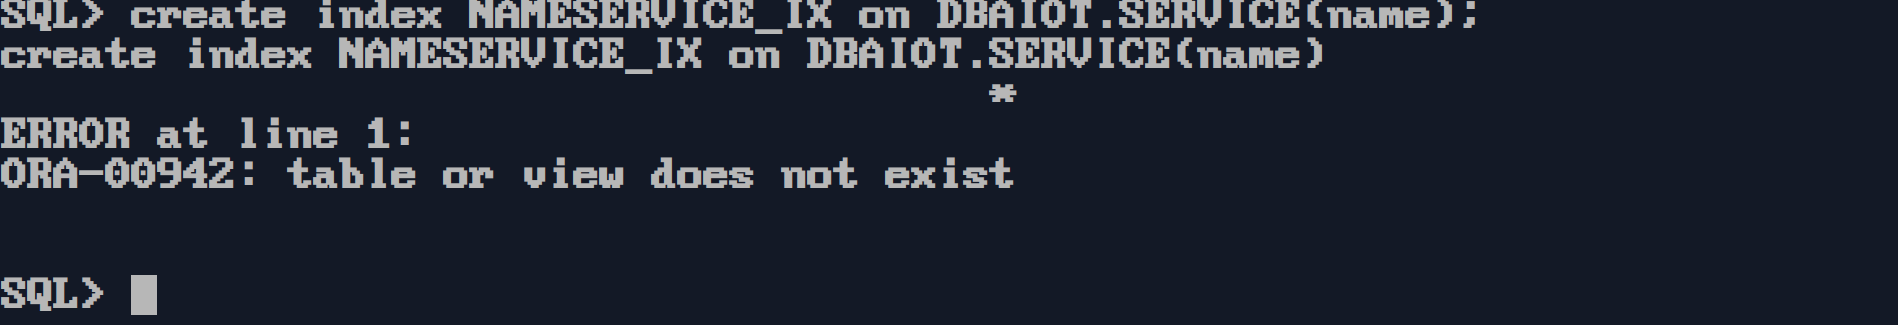
\includegraphics[width=\textwidth]{ScreenShot/Partie4/index.png}
\end{center}

\begin{prettyBox}{}{myblue}
Le problem est que l'admin n'a pas le privelege de select la table DBAIOT.SERVICE ni le privelge de creer des indexes
\end{prettyBox}



\vspace{0.25cm}
\subsubsection*{10.a}
On donne le droit de créer des indexes et selectionner la table DBAIOT.SERVICE a admin depuis DBAIOT

\lstinputlisting[style=sqlstyle]{SQL/Partie4/grant3.sql}

\begin{center}
    
\includegraphics[width=\textwidth]{ScreenShot/Partie4/grant3.png}
\end{center}

\subsubsection*{10.b}
Creation de l'index NAMESERVICE\_IX depuis admin

\lstinputlisting[style=sqlstyle]{SQL/Partie4/index.sql}

\begin{center}
    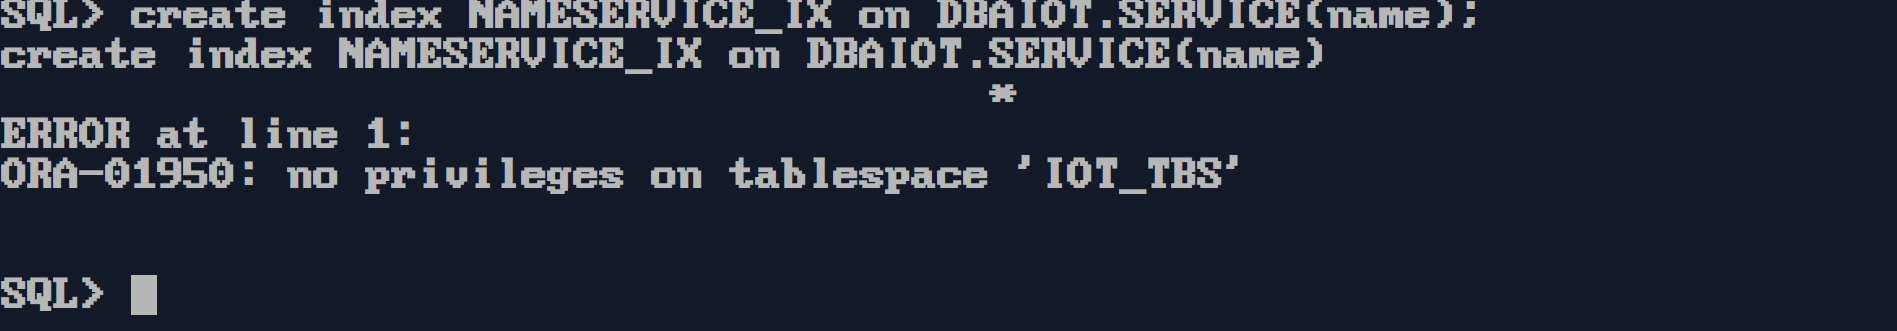
\includegraphics[width=\textwidth]{ScreenShot/Partie4/index1.png}
\end{center}

\begin{prettyBox}{Remarque}{myblue}
\begin{itemize}
\item Admin ne peut pas creer l'index NAMESERVICE\_IX puisqu'il n'a pas les privileges pour ecrire sur la tablespace IOT\_TBS 
\item Admin a pu creer la vue externe USER\_THING car les views externes sont stockes dans la tablespace system
\end{itemize}
\end{prettyBox}



\vspace{0.25cm}
\subsubsection*{11.}

revoker tous les droits qu'on a donner a admin depuis DBAIOT

\lstinputlisting[style=sqlstyle]{SQL/Partie4/revoke.sql}

\begin{center}
    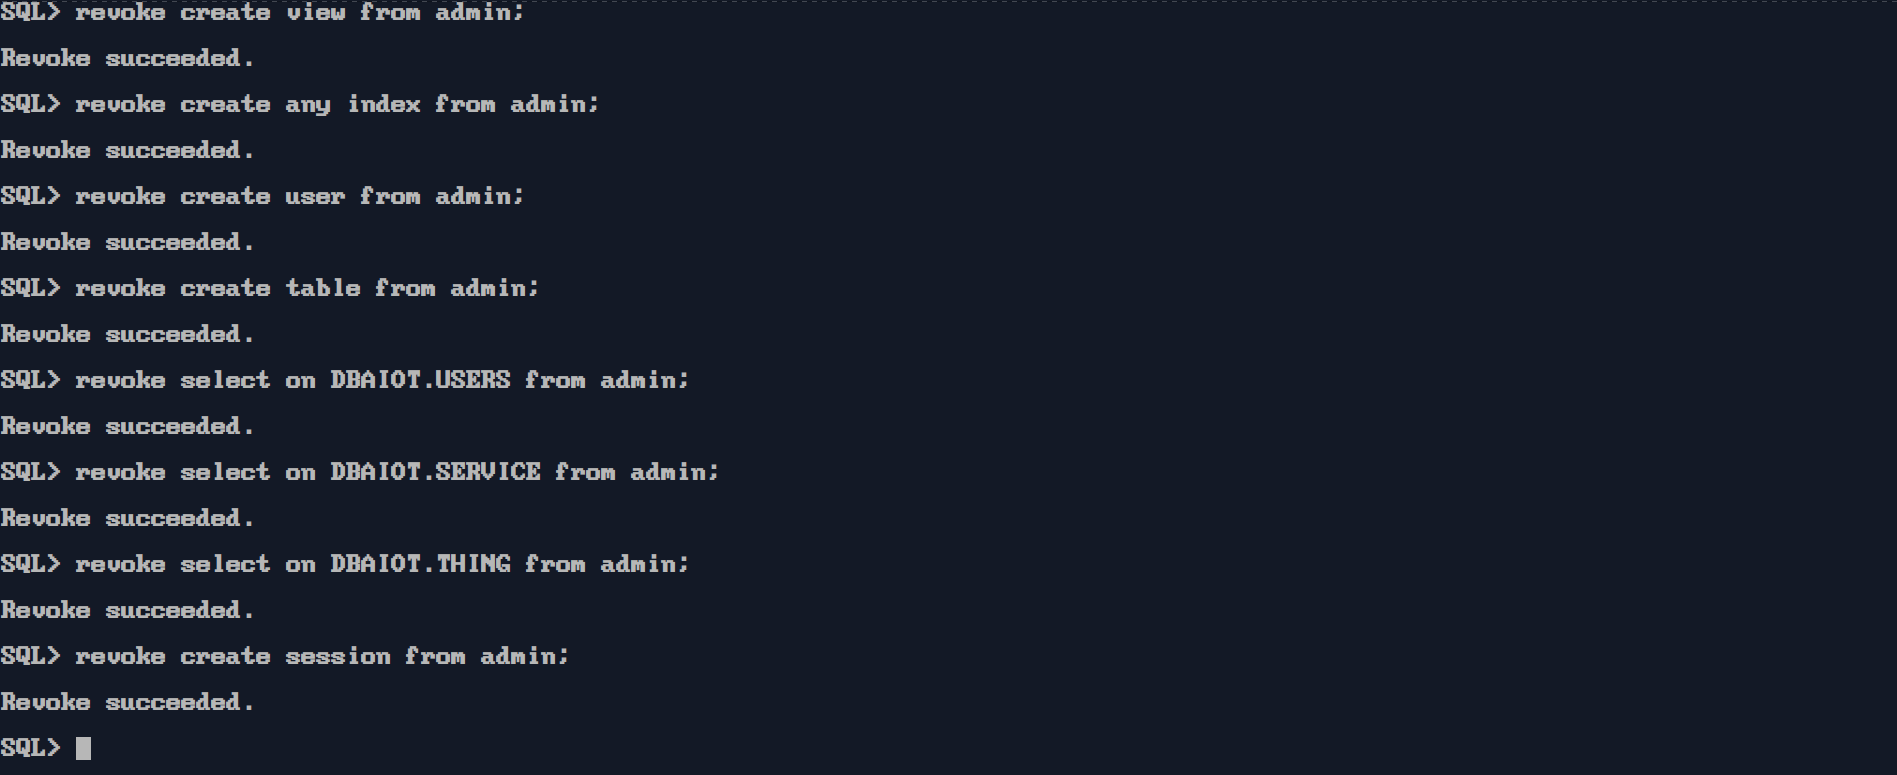
\includegraphics[width=\textwidth]{ScreenShot/Partie4/revoke.png}
\end{center}




\vspace{0.25cm}
\subsubsection*{12.}
On verifie que tous les droits d'admin on ete revoke en selectionnant la table ALL\_TAB\_PRIVS avec garentee='ADMIN' depuis DBAIOT puisque admin n'a plus le droit de creer une session 

\lstinputlisting[style=sqlstyle]{SQL/Partie4/verify2.sql}

\begin{center}
    
\includegraphics[width=\textwidth]{ScreenShot/Partie4/verify2.png}
\end{center}




\vspace{0.25cm}
\subsubsection*{13.}

Création du profil IOT\_Profil, en lui attribuant les limits donner.

\lstinputlisting[style=sqlstyle,basicstyle=\ttfamily\footnotesize]{SQL/Partie4/profile.sql}

\begin{center}
    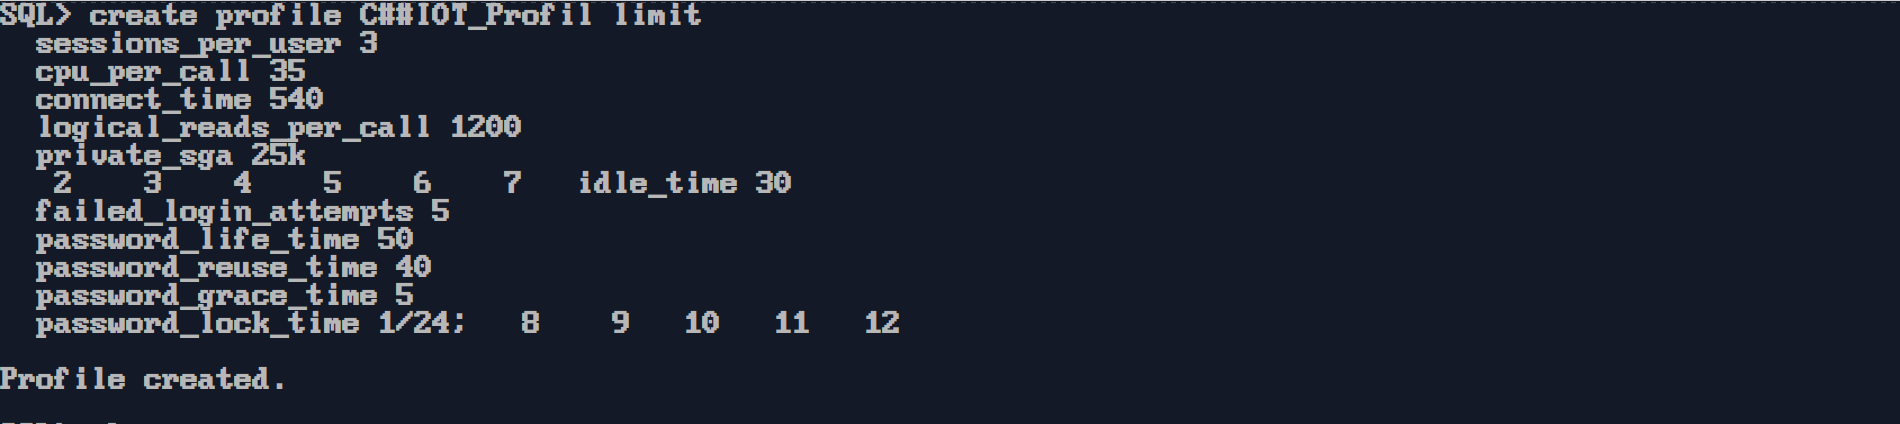
\includegraphics[width=\textwidth]{ScreenShot/Partie4/profile.png}
\end{center}

\begin{prettyBox}{Remarque}{myblue}
J'ai ajouté le préfixe \textbf{C\#\#} parce que je suis dans le conteneur racine \textbf{CDB\$ROOT} de la base de données XE.
\end{prettyBox}



\vspace{0.25cm}
\subsubsection*{14.}
On Affecte le profile IOT\_PROFIL a l'utilisateur admin

\lstinputlisting[style=sqlstyle]{SQL/Partie4/alterprof.sql}

\begin{center}
    
\includegraphics[width=\textwidth]{ScreenShot/Partie4/alterprof.png}
\end{center}




\vspace{0.25cm}
\subsubsection*{15.}
Creation du role SUBSCRIBE\_MANAGER depuis dbaiot en lui donnant les droits demandes

\lstinputlisting[style=sqlstyle]{SQL/Partie4/role.sql}

\begin{center}
    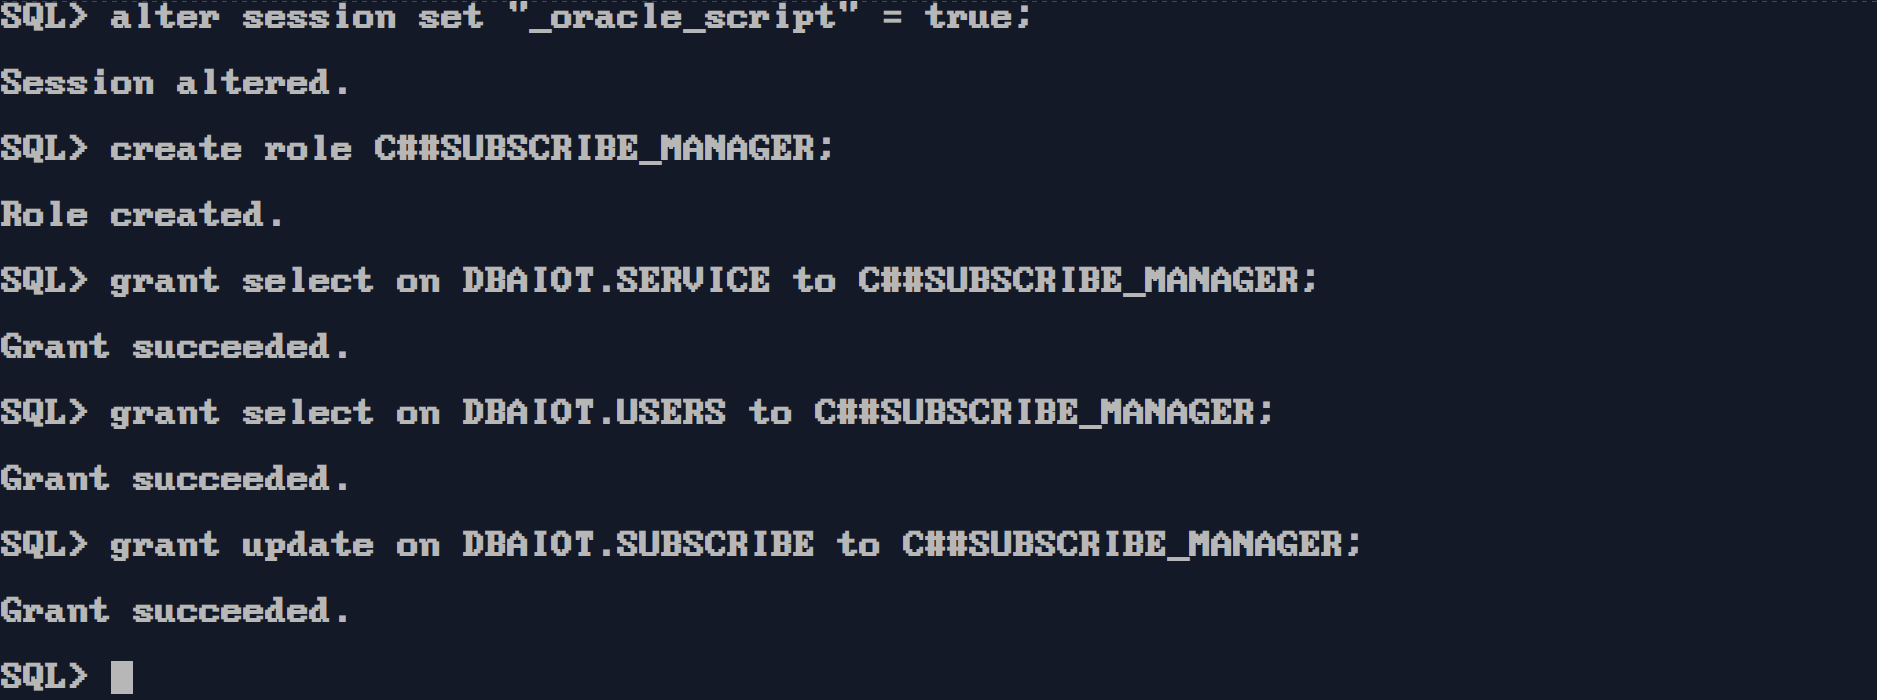
\includegraphics[width=\textwidth]{ScreenShot/Partie4/role.png}
\end{center}




\vspace{0.25cm}
\subsubsection*{16.a}
On affecte le role SUBSCRIBE\_MANAGER a l'utilisateur admin

\lstinputlisting[style=sqlstyle]{SQL/Partie4/grantrole.sql}

\begin{center}
    
\includegraphics[width=\textwidth]{ScreenShot/Partie4/grantrole.png}
\end{center}

\subsubsection*{16.b}
les role des utilisteur sont stockes dans les table USER\_ROLE\_PRIVS et DBA\_ROLE\_PRIVS , probleme et que
admin ne peut pas creer de session donc on ne peut pas se connecter en tant que admin et afficher USER\_ROLE\_PRIVS
, et dbaiot n'est pas DBA pour acceder a DBA\_ROLE\_PRIVS , donc on se connect en tant que sysdba et afficher  
DBA\_ROLE\_PRIVS  avec WHERE GRANTEE = 'ADMIN' pour afficher just celle d'admin

\lstinputlisting[style=sqlstyle]{SQL/Partie4/verifyrole.sql}

\begin{center}
    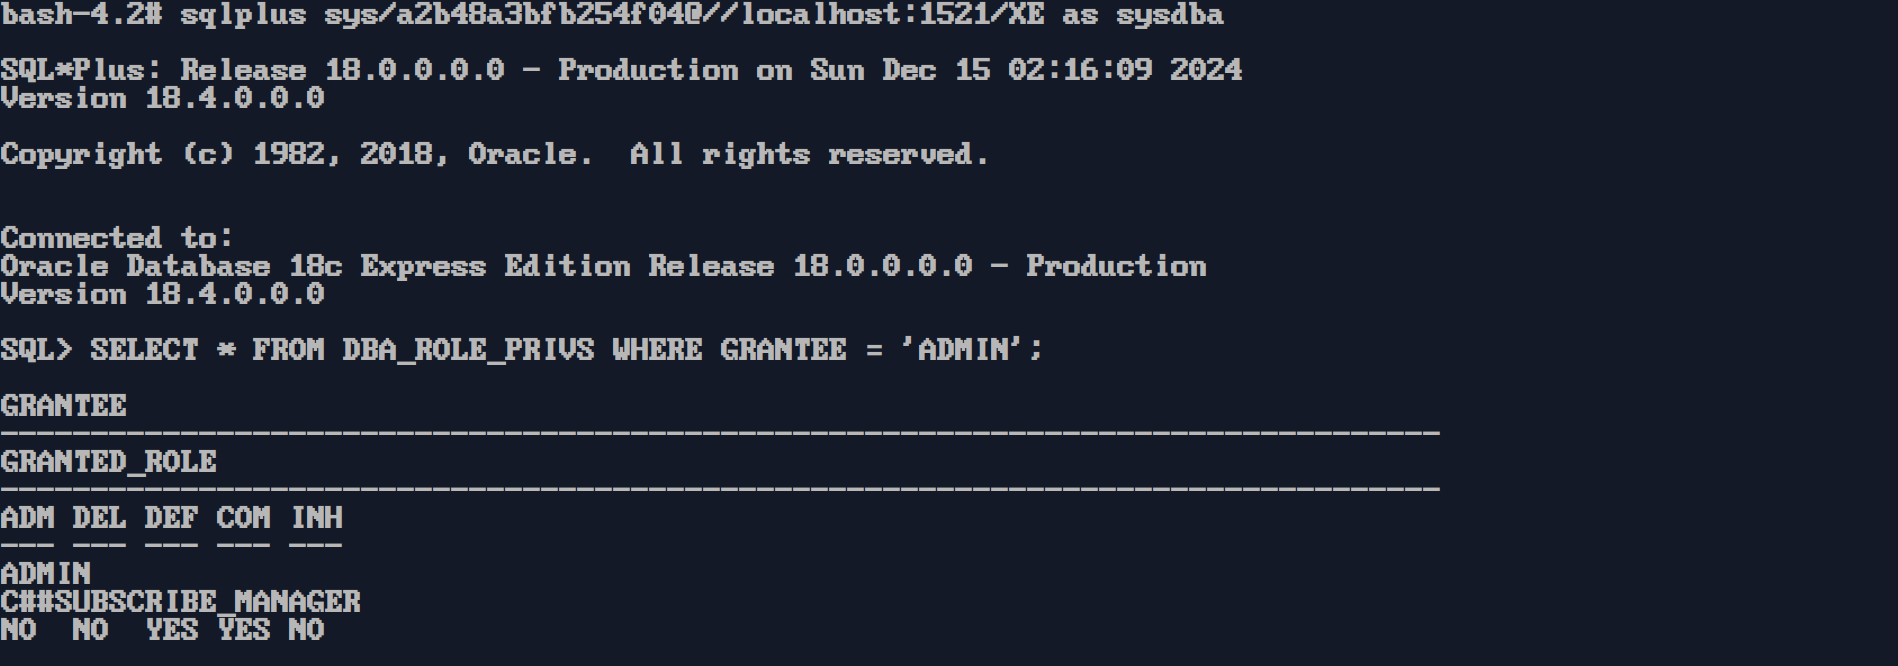
\includegraphics[width=\textwidth]{ScreenShot/Partie4/verifyrole.png}
\end{center}

\begin{prettyBox}{}{myblue}
Depuis l'output on remarque que admin a le role C\#\#SUBSCRIBE\_MANAGER
\end{prettyBox}





\vspace{0.25cm}
\subsection*{\underline{Partie 5}}
\subsubsection*{1.a}
On se connect en tant que system

\lstinputlisting[style=sqlstyle]{SQL/Partie5/connectsystem.sql}

\begin{center}
    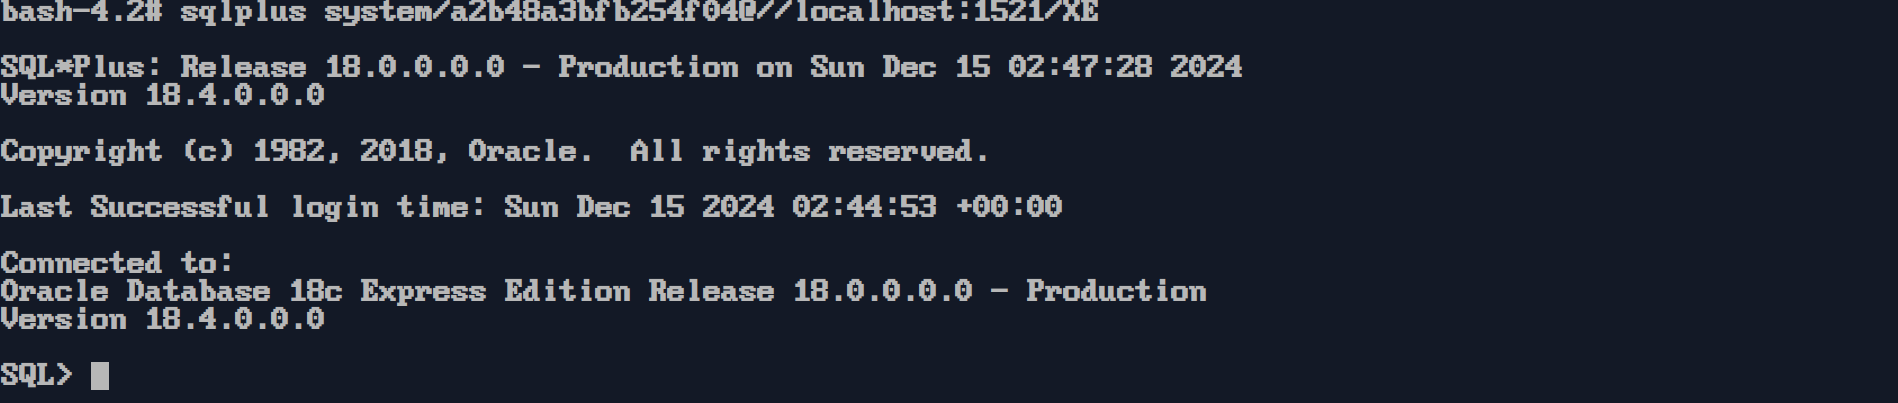
\includegraphics[width=\textwidth]{ScreenShot/Partie5/connectsystem.png}
\end{center}

\newpage
\subsubsection*{1.b}
On affiche la structure de la table dict en utilisant desc

\lstinputlisting[style=sqlstyle]{SQL/Partie5/dict.sql}

\begin{center}
    
\includegraphics[width=\textwidth]{ScreenShot/Partie5/dict.png}
\end{center}

\subsubsection*{1.c}
On affiche la table dict , elle a 4623 instances

\lstinputlisting[style=sqlstyle]{SQL/Partie5/selectDICT.sql}

\begin{center}
    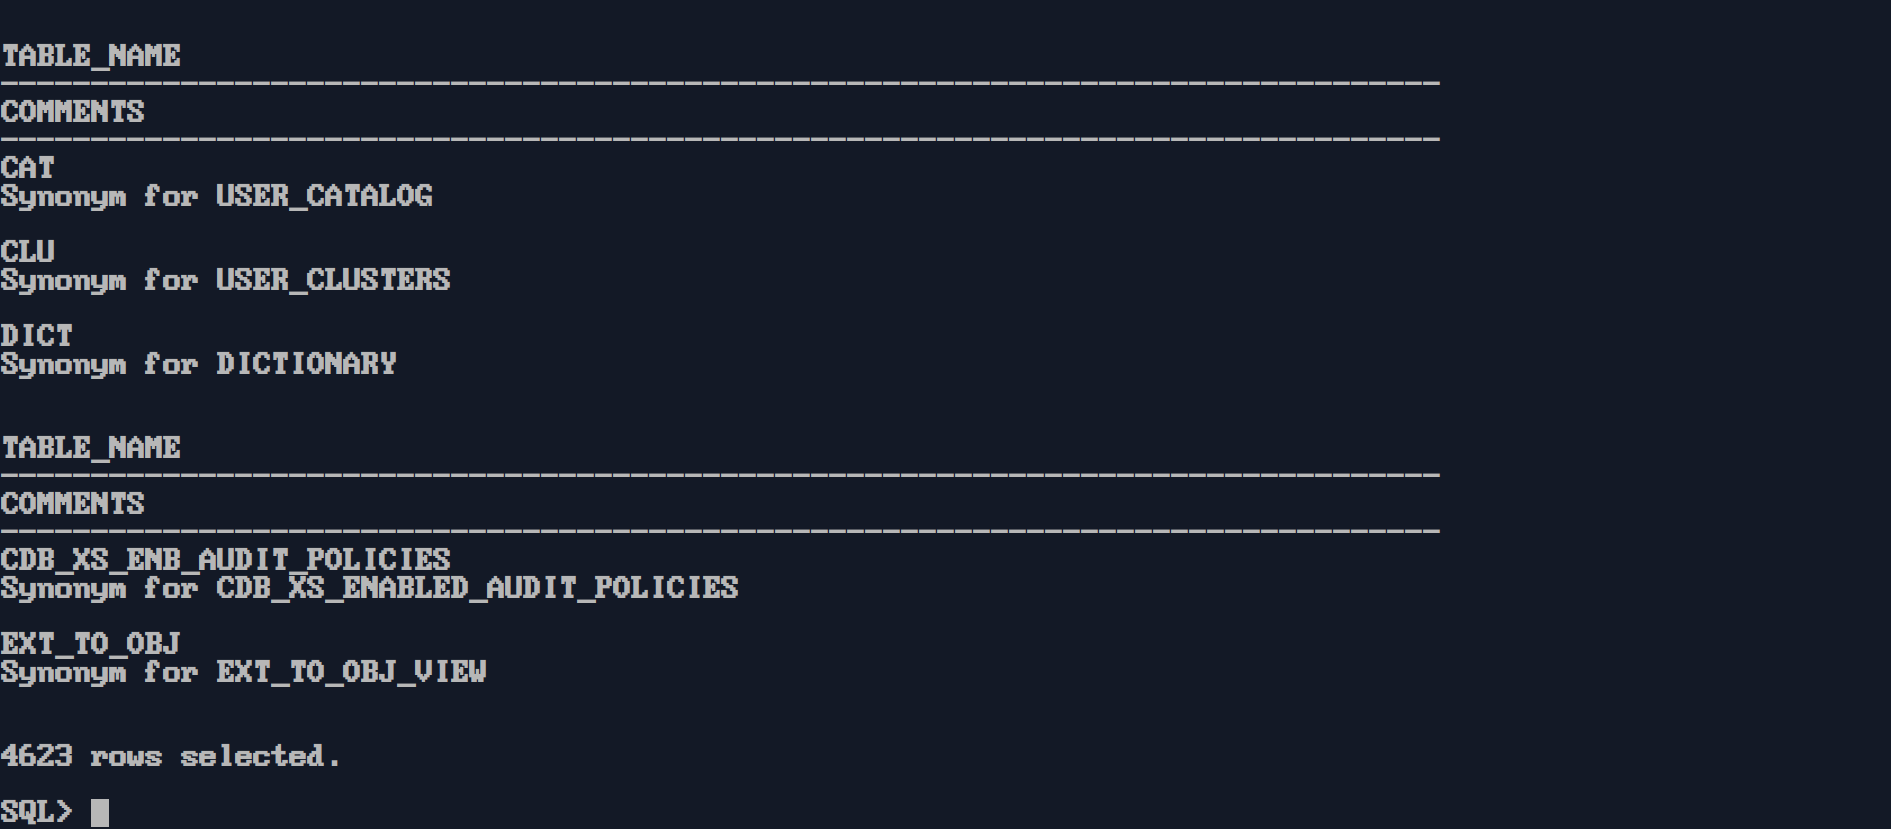
\includegraphics[width=\textwidth]{ScreenShot/Partie5/selectDICT.png}
\end{center}



\vspace{0.25cm}
\subsubsection*{\underline{Experimental}}
\begin{tabular}{|c|c|c|c|c|c|c|c|c|c|c|c|c|c|c|}
    \hline
    N & \(10^3\) & \(2.10^3\) & \(10^4\) & \(2.10^4\) & \(10^5\) & \(2.10^5\) & \(10^6\) & \(2.10^6\) & \(10^7\) & \(2.10^7\) & \(10^8\) & \(2.10^8\) & \(10^9\) & \(2.10^9\) \\
    \hline
    \makecell{Time\\\((10^{-5})\)} & 8 & 9.8 & 10.8 & 19.4 & 33.6 & 59.3 & 261.1 & 505.7 & 2458.4 & 5071.6 & 24458.7 & 48759.0 & 243312.2 & 487828.6 \\
    \hline
\end{tabular}



\vspace{1cm}

\newpage

\subsubsection*{\underline{Theoritical}}
We first need to find  \(\Delta t\) , for that we will take one runtime value from the experimental study and solve a simple equation 

\vspace{0.15cm}

for n = \(10^4\) and execution time T(n) = \(10.8\times10^{-5}\) :

\vspace{0.75cm}
\begin{align*}
&f(n)\times\Delta t = T(n)\\[0.15cm]
&\Delta t = \frac{T(n)}{f(n)} \\[0.15cm]
&\Delta t = \frac{T(n)}{5n + 6}\\[0.15cm]
&\Delta t = \frac{10.8\times10^{-5}}{5\times 10^4 + 6} \\[0.15cm]
&\Delta t = 2.1597408311\times10^{-9} \\[0.25cm]
&\boxed{\Delta t \approx 2.16\times10^{-9}}
\end{align*}





\vspace{2cm}
\begin{tabular}{|c|c|c|c|c|c|c|c|c|c|c|c|c|c|c|c|c|}
    \hline
    N & \(10^3\) & \(2.10^3\) & \(10^4\) & \(2.10^4\) & \(10^5\) & \(2.10^5\) & \(10^6\) & \(2.10^6\) & \(10^7\) & \(2.10^7\) & \(10^8\) & \(2.10^8\) & \(10^9\) & \(2.10^9\) & \(10^{10}\) & \(2.10^{10}\) \\
    \hline
    \makecell{Time\\\((10^{-5})\)} & 1.08 & 2.16 & 10.08 & 21.6 & 108 & 216 & 1080 & 2160 & 10800 & 21600 & \makecell{108\\\(\times10^3\)} & \makecell{216\\\(\times10^3\)} & \makecell{108\\\(\times10^4\)} & \makecell{216\\\(\times10^4\)} & \makecell{108\\\(\times10^5\)} & \makecell{216\\\(\times10^5\)}\\
    \hline
\end{tabular}



\vspace{0.25cm}
\lstinputlisting[style=cstyle]{Questions/Part4/prime4.c}

\subsubsection*{\underline{Experimental}}

\begin{tabular}{|c|c|c|c|c|c|c|c|c|c|c|}
\hline
N & 1000003 & 2000003 & 4000037 & 8000009 & 16000057 & 32000011 & 64000031 & 128000003 & 256000001 & 512000009 \\
\hline
\makecell{T(n)\\\(10^{-5}\)} & 6.5 & 7.4 & 7.5 & 7.8 & 8.5 & 8.7 & 11.2 & 11.4 & 13.8 & 14.5\\
\hline
\end{tabular}

\vspace{0.25cm}

\begin{tabular}{|c|c|c|}
    \hline
    N & 1024000009 & 2048000011\\
    \hline
    \makecell{T(n)\\\(10^{-5}\)}  & 17.1 & 19\\
    \hline
\end{tabular}



\vspace{0.5cm}

\begin{figure}[h!]
    \centering
    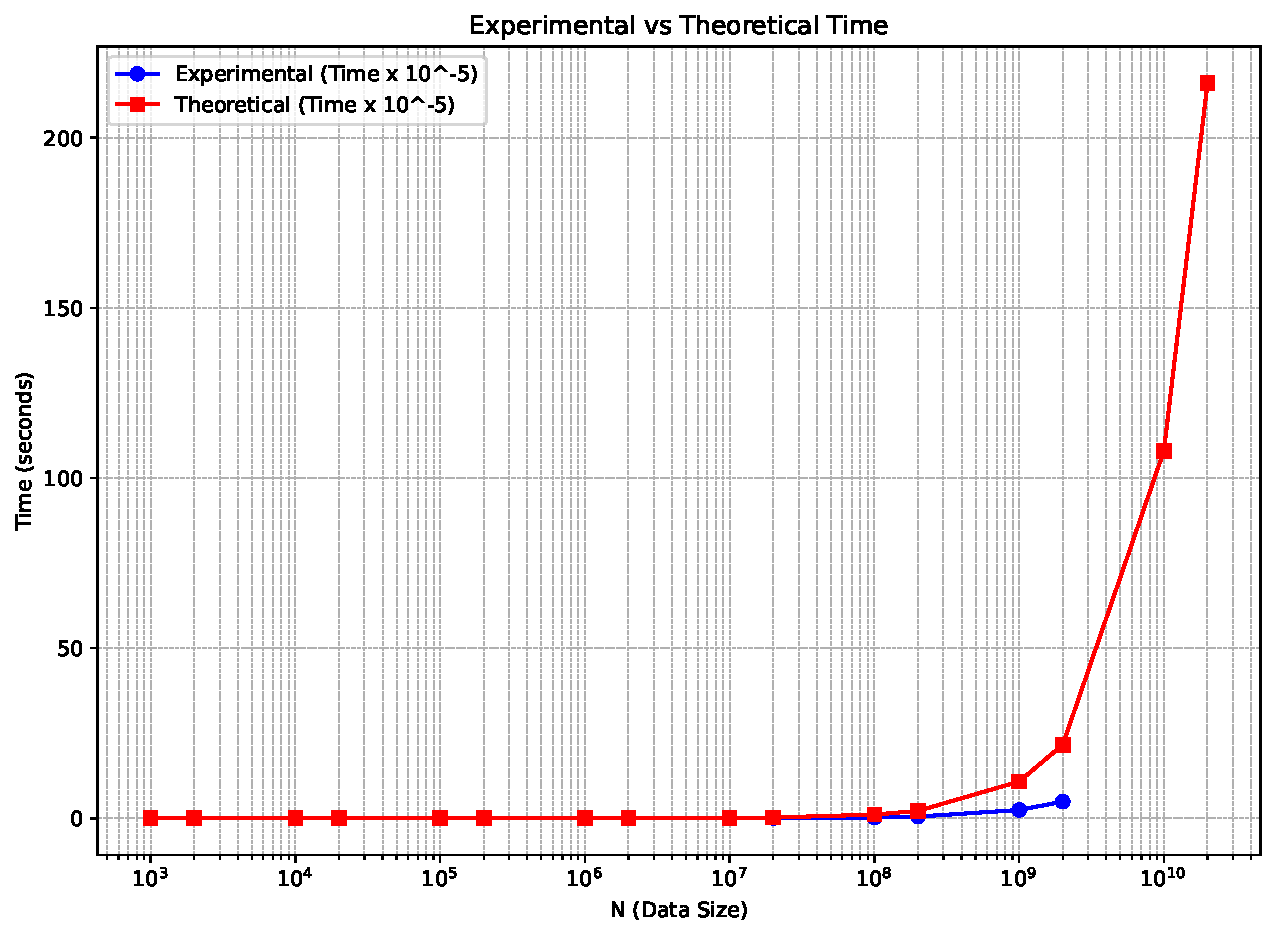
\includegraphics[width=0.85\textwidth]{Questions/Part4/plot.pdf}
    \label{fig:time_plot}
\end{figure}

\newpage

To Draw the plots i used the below python script :

\vspace{1cm}

\lstinputlisting[style=pythonstyle2,inputencoding=utf8]{Questions/Part4/draw.py}

\vspace{1cm}

\begin{prettyBox}{Observation}{greenPlot}
From the plots we notice that the 4th solution takes about the same time as 3rd solution but as n grows bigger the 4th solution takes about
half time of the 3rd therefore the 4th solution is the most efficient out of all the solutions
\end{prettyBox}




\vspace{0.25cm}

\lstinputlisting[style=cstyle]{Questions/Part1/PSUM\_1.c}


\vspace{0.25cm}
\section{Transfert Du Fichier Malveillant}

\begin{center}
    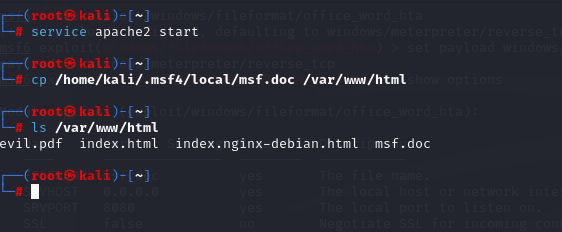
\includegraphics[width=0.8\textwidth]{Question/SC/9_kali.PNG}
\end{center}

\vspace{0.15cm}

\begin{center}
    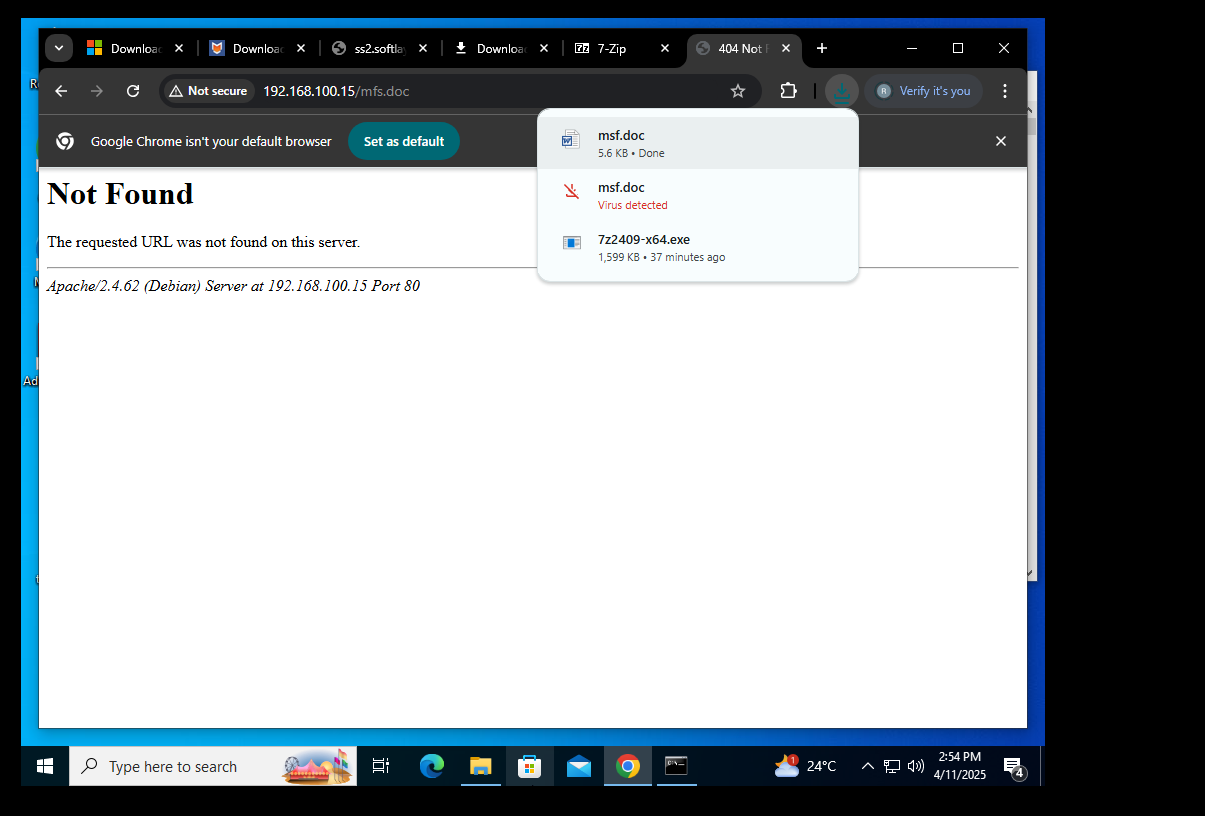
\includegraphics[width=0.6\textwidth]{Question/SC/9_win.PNG}
\end{center}

\vspace{0.15cm}

\begin{center}
    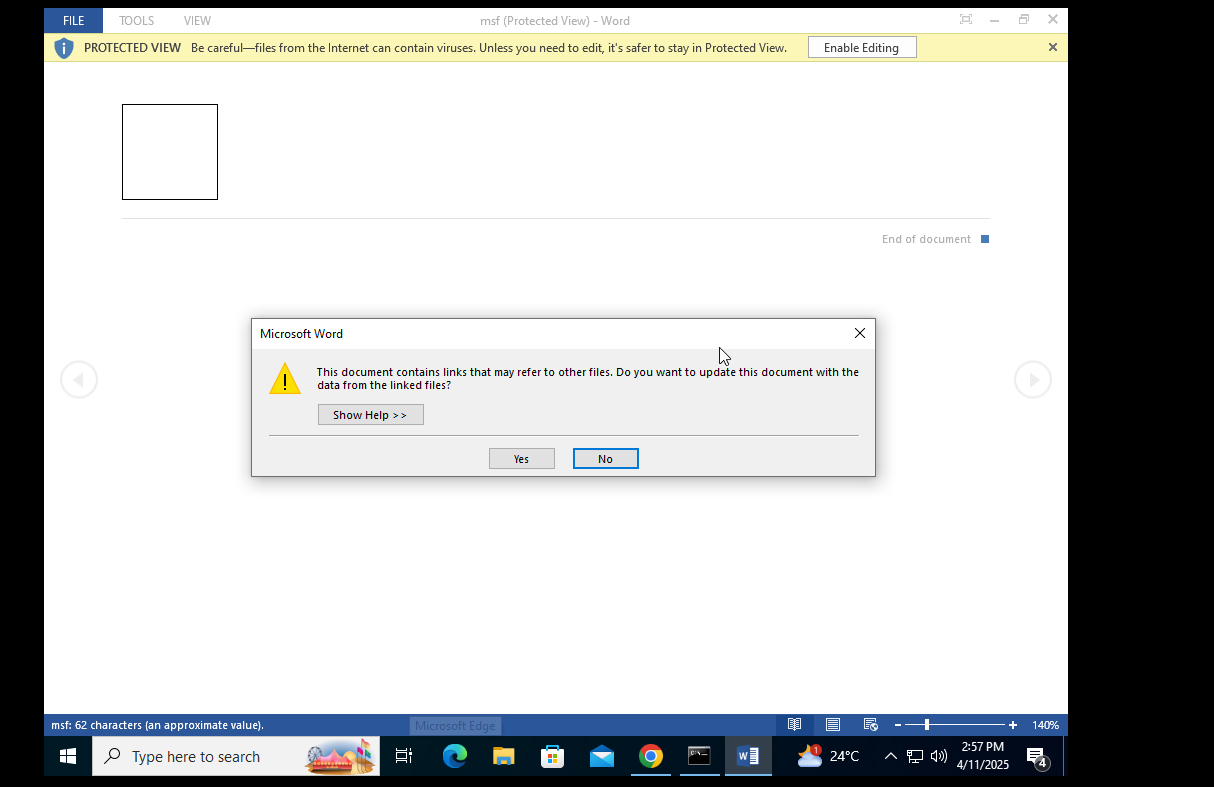
\includegraphics[width=0.6\textwidth]{Question/SC/9_3.PNG}
\end{center}


\vspace{0.35cm}

\begin{prettyBox}{Transfert de fichiers malveillants}{myblue}
\begin{itemize}
    \item On peut transférer le fichier à l'utilisateur sous un nom différent par email, lien, programme qui force l'installation, etc.
\end{itemize}
\end{prettyBox}


\vspace{0.25cm}
\section{Payload \& Handler}

\begin{center}
    \includegraphics[width=0.8\textwidth]{Question/SC/13_14_15-.PNG}
\end{center}

\vspace{0.15cm}

\begin{center}
    \includegraphics[width=0.6\textwidth]{Question/SC/16.PNG}
\end{center}

\vspace{0.15cm}

\begin{center}
    \includegraphics[width=0.6\textwidth]{Question/SC/17.PNG}
\end{center}

\vspace{0.15cm}
\begin{center}
    \includegraphics[width=0.6\textwidth]{Question/SC/18.PNG}
\end{center}


\vspace{0.35cm}


\begin{prettyBox}{Définitions Des Termes}{myblue}
    \begin{itemize}
        \item \textbf{Handler} : programme exécuté sur la machine de l'attaquant, qui se met en écoute afin d'attendre une connexion provenant de la victime lorsqu'elle exécute le payload (par exemple, en ouvrant un lien ou un fichier malveillant).
        \item \textbf{Payload} : programme malveillant exécuté sur la machine de la victime suite à une action spécifique réalisée par celle-ci.
        \item \textbf{Reverse Shell} : mécanisme permettant à l'attaquant d'exécuter des commandes shell sur la machine de la victime depuis sa propre machine, en utilisant une connexion TCP inverse initiée par la victime.
        \item \textbf{Message affiché} : message qui apparaît sur la machine de la victime, identique à celui configuré précédemment via la commande \texttt{set LAUNCH\_MESSAGE}.
    \end{itemize}
\end{prettyBox}



\vspace{0.25cm}
\section{Reverse\_Shell}

\begin{center}
    \includegraphics[width=0.8\textwidth]{Question/SC/18_kali.PNG}
\end{center}

\vspace{0.15cm}

\begin{center}
    \includegraphics[width=0.6\textwidth]{Question/SC/19_0.PNG}
\end{center}

\vspace{0.15cm}

\begin{center}
    \includegraphics[width=0.6\textwidth]{Question/SC/19.PNG}
\end{center}

\vspace{0.15cm}
\begin{center}
    \includegraphics[width=0.6\textwidth]{Question/SC/19_2.PNG}
\end{center}

\vspace{0.15cm}
\begin{center}
    \includegraphics[width=0.6\textwidth]{Question/SC/20_1.PNG}
\end{center}

\vspace{0.15cm}
\begin{center}
    \includegraphics[width=0.6\textwidth]{Question/SC/20_2.PNG}
\end{center}



\vspace{0.35cm}


\begin{prettyBox}{Commandes \& Remarques}{myblue}
    \begin{itemize}
        \item \textbf{Remarque} : Après que l'utilisateur ouvre le fichier \texttt{template.pdf}, le payload s'exécute et l'on peut alors démarrer une session de type \texttt{reverse\_shell}.
        \item \textbf{pwd} : affiche le répertoire courant sur la machine cible.
        \item \textbf{keyboard\_send} : cette commande écrit le message spécifié par l'attaquant directement sur la machine victime. Dans notre cas, le message apparaît dans le bloc-notes (\texttt{notepad.exe}).
        \item \textbf{ps} : affiche les noms, les identifiants (PID), et les chemins d'accès des processus actifs sur la machine cible.
    \end{itemize}
\end{prettyBox}



\vspace{0.25cm}
\subsubsection*{8.}
Pour vérifier s'il y a une référence de la table \texttt{SUBSCRIBE} dans la table \texttt{THING},
nous allons effectuer une jointure de la table \texttt{USER\_CONSTRAINTS} avec elle-même. Nous 
utilisons un \textit{select imbriqué} ou la \textit{sous-requête} récupère les noms
des contraintes référencées de la table \texttt{THING}, c'est-à-dire les contraintes de clé
primaire des table references par \texttt{THING}. La requête principale compte ensuite le nombre de contraintes de 
clé primaire dans la table \texttt{SUBSCRIBE} qui figurent parmi les contraintes obtenues dans la sous-requête. 
si count = 0 , pas de references sinon si 1 ya une reference 

\lstinputlisting[style=sqlstyle]{SQL/Partie5/fr.sql}

\begin{center}
    \includegraphics[width=\textwidth]{ScreenShot/Partie5/fr.png}
\end{center}

\begin{prettyBox}{Remarque}{myblue}
\begin{itemize}
    \item Constraint\_Type = 'R' : contrainte cle etrangere
    \item Constraint\_Type = 'P' : contrainte cle primaire
    \item R\_Constraint\_Name : nom des contrainte cle primaire reference par la table
\end{itemize}
\end{prettyBox}




\vspace{0.25cm}
\subsubsection*{9.}
Pour afficher les contraintes creer par DBAIOT on va utiliser la table USER\_CONSTRAINTS , et
afficher les noms des contraintes(constraint\_name) , type (constraint\_name) , les tables associe (table\_name)

\lstinputlisting[style=sqlstyle]{SQL/Partie5/const.sql}

\begin{center}
    \includegraphics[width=\textwidth]{ScreenShot/Partie5/const.png}
\end{center}





\vspace{0.25cm}
\subsubsection*{10.a}
On va afficher les id(column\_id) , nom(column\_name) , type de donnes(data\_type) , nullabilite(nullable) , valeur par defaut(data\_default)
des attributs de la table SUBSCRIBE en utilisant la table USER\_TAB\_COLUMNS et bien sure le where pour just selectionner la table SUBSCRIBE
where table\_name='SUBSCRIBE'

\lstinputlisting[style=sqlstyle]{SQL/Partie5/att.sql}

\begin{center}
    \includegraphics[width=\textwidth]{ScreenShot/Partie5/att.png}
\end{center}

\subsubsection*{10.b}
Pour obtenir le nom de la contrainte cle primaire et les nom de ces attributs  on va faire
une jointure entre USER\_CONSTRIANTS et USER\_CONS\_COLUMNS , la premiere table va nous aider
a filterer les contraintes pour just avoir des contraintes de type cle primaire \\t1.constraint\_type = 'P' 
de la table SUBSCRIBE t1.table\_name='SUBSCRIBE' puis on utilise la deuxieme table pour afficher les noms des attributs de la cle primaire
t2.column\_name avec la jointure t1.constraint\_name=t2.constraint\_name

\lstinputlisting[style=sqlstyle]{SQL/Partie5/pk.sql}

\begin{center}
    \includegraphics[width=\textwidth]{ScreenShot/Partie5/pk.png}
\end{center}

\subsubsection*{10.c}
Pour afficher les nom des contraintes cle etrangers et le nom de l'attribut , table reference , colonne reference on doit utiliser des imbriquation de select 
toujours avec les deux table USER\_CONSTRIANTS et USER\_CONS\_COLUMNS , le outer select fait une jointure entre les tables et affiche le nom de la contrainte
et son attribut en filtron le type pour foreign key t1.constraint\_type = 'R' de la table SUBSCRIBE t1.table\_name='SUBSCRIBE' , pour afficher la table reference
on va selectioner le nom de la table de la contrainte cle primaire reference par la table SUBSCRIBE t1.r\_constraint\_name=t11.constraint\_name depuis la table
USER\_CONSTRAINTS, pour affiche les colonnes reference
en selectionne les nom des colonnes de la contrainte cle primaire reference par la table SUBSCRIBE de puis la table USER\_CONS\_COLUMNS t1.r\_constraint\_name=t22.constraint\_name 

\lstinputlisting[style=sqlstyle]{SQL/Partie5/fr1.sql}

\begin{center}
    \includegraphics[width=\textwidth]{ScreenShot/Partie5/fr1.png}
\end{center}

\subsubsection*{10.d}
Pour obtenir les nom des contraintes uniques et les nom des attributs associes on va faire
une jointure entre USER\_CONSTRIANTS et USER\_CONS\_COLUMNS , la premiere table va nous aider
a filterer les contraintes pour just avoir des contraintes de type unique \\t1.constraint\_type = 'U' 
de la table SUBSCRIBE t1.table\_name='SUBSCRIBE' puis on utilise la deuxieme table pour afficher le nom de l'attribut unique
t2.column\_name avec la jointure t1.constraint\_name=t2.constraint\_name

\lstinputlisting[style=sqlstyle]{SQL/Partie5/uni.sql}

\begin{center}
    \includegraphics[width=\textwidth]{ScreenShot/Partie5/uni.png}
\end{center}

\subsubsection*{10.e}
On va obtenir les nom des contraints check + leur condition avec la table
USER\_CONSTRAINTS , on selectionnant l'attribut constraint\_name(nom de la contraint) ,
search\_condition(condition du check) et pour avoir que les contraintes de la table subscribe de type check
on utilise le where clause table\_name='SUBSCRIBE' and constraint\_type='C'(type check)

\lstinputlisting[style=sqlstyle]{SQL/Partie5/chk.sql}

\begin{center}
    \includegraphics[width=\textwidth]{ScreenShot/Partie5/chk.png}
\end{center}







\vspace{0.25cm}
\subsubsection*{11.a}
On donne 2 privilegs system a admin(creation session,user) et 1 privilege objet
(select on DBAIOT.USERS) depuis DBAIOT

\lstinputlisting[style=sqlstyle]{SQL/Partie5/grant.sql}

\begin{center}
    \includegraphics[width=\textwidth]{ScreenShot/Partie5/grant.png}
\end{center}

\subsubsection*{11.b}
On se connect d'abord en tant qu'admin

\lstinputlisting[style=sqlstyle]{SQL/Partie5/connectadmin.sql}

Pour afficher les privileges on va utilise la table USER\_TAB\_PRIV
pour les privileges objets et la table USER\_SYS\_PRIV pour les privileges
system 

\lstinputlisting[style=sqlstyle]{SQL/Partie5/priv.sql}

\begin{center}
    \includegraphics[width=\textwidth]{ScreenShot/Partie5/objpriv.png}
\end{center}

\begin{center}
    \includegraphics[width=\textwidth]{ScreenShot/Partie5/syspriv.png}
\end{center}

\begin{prettyBox}{Remarque}{myblue}
On remarque que admin a comme droits system :
\begin{itemize}
    \item creation session
    \item creation user
\end{itemize}

Et comme droits object :
\begin{itemize}
    \item select on DBAIOT.USERS
\end{itemize}
\end{prettyBox}




\vspace{0.25cm}
\subsubsection*{12.}
Pour afficher les roles d'admin on va utiliser la table USER\_ROLE\_PRIVS et just afficher 
l'attribut granted\_name (nom du role) depuis admin

\lstinputlisting[style=sqlstyle]{SQL/Partie5/role.sql}

\begin{center}
    \includegraphics[width=\textwidth]{ScreenShot/Partie5/role.png}
\end{center}

\begin{prettyBox}{Remarque}{myblue}
Le role C\#\#SUBSCRIBE\_MANAGER a ete creer dans la partie4
\end{prettyBox}



\vspace{0.25cm}
\subsubsection*{13.}
Pour afficher les objets dont ADMIN est propriétaire on va utiliser
la table ALL\_OBJECTS , selectionner l'attribut OBJECT\_NAME et filtrer avec
where owner='ADMIN' pour seulement avoir les objets d'ADMIN

\lstinputlisting[style=sqlstyle]{SQL/Partie5/obj.sql}

\begin{center}
    \includegraphics[width=\textwidth]{ScreenShot/Partie5/obj.png}
\end{center}

\begin{prettyBox}{Remarque}{myblue}
L'objet USER\_THING est une vue qu'on a creer dans la partie4
\end{prettyBox}



\vspace{0.25cm}
\subsubsection*{14.}
Pour trouver le propriétaire de la table SUBSCRIBE, on va afficher
l'attribut OWNER de la table ALL\_OBJECTS et filtre avec where
object\_name='SUBSCRIBE' pour seulement avoir le propietaire de la table SUBSCRIBE

\lstinputlisting[style=sqlstyle]{SQL/Partie5/own.sql}

\begin{center}
    \includegraphics[width=\textwidth]{ScreenShot/Partie5/own.png}
\end{center}





\vspace{0.25cm}
\subsubsection*{15.}
Pour afficher la taille de la table SUBSCRIBE en KO , on va selectionner la table
USER\_SEGMENTS depuis DBAIOT , affichant l'attribut BYTES qui donne la taille du segment
en byte(octet) en va le diviser sur \(2^{10}\)(1024) pour converitre au KO et en filtre avec
where segment\_name='SUBSCRIBE' pour just avoir la taille de la table SUBSCRIBE

\lstinputlisting[style=sqlstyle]{SQL/Partie5/size.sql}

\begin{center}
    \includegraphics[width=\textwidth]{ScreenShot/Partie5/size.png}
\end{center}





\vspace{0.25cm}
\subsubsection*{16.a}
Creer utilisateur Test et lui donner tous les droits

\lstinputlisting[style=sqlstyle]{SQL/Partie5/create.sql}

\begin{center}
    \includegraphics[width=\textwidth]{ScreenShot/Partie5/create.png}
\end{center}

\subsubsection*{16.b}
Connecter en tant que Test

\lstinputlisting[style=sqlstyle]{SQL/Partie5/connecttest.sql}

\begin{center}
    \includegraphics[width=\textwidth]{ScreenShot/Partie5/connecttest.png}
\end{center}

\subsubsection*{16.c}

On va afficher les tables USER\_OBJECTS , USER\_TAB\_COLUMNS , USER\_CONSTRAINTS 
avant et apres des query DDL


\lstinputlisting[style=sqlstyle]{SQL/Partie5/testobj.sql}

\begin{center}
    \includegraphics[width=\textwidth]{ScreenShot/Partie5/testobj1.png}
\end{center}


\lstinputlisting[style=sqlstyle]{SQL/Partie5/testatt.sql}

\begin{center}
    \includegraphics[width=\textwidth]{ScreenShot/Partie5/testatt1.png}
\end{center}


\lstinputlisting[style=sqlstyle]{SQL/Partie5/const.sql}

\begin{center}
    \includegraphics[width=\textwidth]{ScreenShot/Partie5/testconst1.png}
\end{center}

\begin{prettyBox}{Remarque}{myblue}
Puisque test n'a jamais creer de contraints , attribut, objets toute les tables renvoit 0 lignes
\end{prettyBox}

On va creer deux Table t1 et t2

\lstinputlisting[style=sqlstyle]{SQL/Partie5/tab.sql}


\begin{center}
    \includegraphics[width=\textwidth]{ScreenShot/Partie5/tab.png}
\end{center}


On va afficher les object et attribut de Test
\lstinputlisting[style=sqlstyle]{SQL/Partie5/testobj.sql}

\begin{center}
    \includegraphics[width=\textwidth]{ScreenShot/Partie5/testobj2.png}
\end{center}


\lstinputlisting[style=sqlstyle]{SQL/Partie5/testatt.sql}

\begin{center}
    \includegraphics[width=\textwidth]{ScreenShot/Partie5/testatt2.png}
\end{center}

\begin{prettyBox}{Remarque}{myblue}
On remarque apres la creation des deux tables , les tables USER\_OBJECTS , USER\_TAB\_COLUMNS on ete mise a jour
\end{prettyBox}

\vspace{0.25cm}
On va ajouter une colonne a t1 puis afficher les attributes de Test

\lstinputlisting[style=sqlstyle]{SQL/Partie5/col.sql}

\begin{center}
    \includegraphics[width=\textwidth]{ScreenShot/Partie5/col.png}
\end{center}

\lstinputlisting[style=sqlstyle]{SQL/Partie5/testatt.sql}

\begin{center}
    \includegraphics[width=\textwidth]{ScreenShot/Partie5/testatt3.png}
\end{center}

\begin{prettyBox}{Remarque}{myblue}
On appercoie que l'attribut name a ete ajoute a la table USER\_TAB\_COLUMNS et avec sa valeur par defaut 'admin'
\end{prettyBox}

\vspace{0.25cm}
On va ajouter une contraint de cle primaire pour t1 et une unique pour t2
\lstinputlisting[style=sqlstyle]{SQL/Partie5/con.sql}

\begin{center}
    \includegraphics[width=\textwidth]{ScreenShot/Partie5/con.png}
\end{center}

\lstinputlisting[style=sqlstyle]{SQL/Partie5/testatt.sql}

\begin{center}
    \includegraphics[width=\textwidth]{ScreenShot/Partie5/testconst2.png}
\end{center}

\begin{prettyBox}{Remarque}{myblue}
On remarque qu'apres avoir ajouter les contraintes la table USER\_CONSTRAINTS a ete misajour
\end{prettyBox}















\end{document}


